\documentclass{article}\usepackage[]{graphicx}\usepackage[]{color}
% maxwidth is the original width if it is less than linewidth
% otherwise use linewidth (to make sure the graphics do not exceed the margin)
\makeatletter
\def\maxwidth{ %
  \ifdim\Gin@nat@width>\linewidth
    \linewidth
  \else
    \Gin@nat@width
  \fi
}
\makeatother

\definecolor{fgcolor}{rgb}{0.345, 0.345, 0.345}
\newcommand{\hlnum}[1]{\textcolor[rgb]{0.686,0.059,0.569}{#1}}%
\newcommand{\hlstr}[1]{\textcolor[rgb]{0.192,0.494,0.8}{#1}}%
\newcommand{\hlcom}[1]{\textcolor[rgb]{0.678,0.584,0.686}{\textit{#1}}}%
\newcommand{\hlopt}[1]{\textcolor[rgb]{0,0,0}{#1}}%
\newcommand{\hlstd}[1]{\textcolor[rgb]{0.345,0.345,0.345}{#1}}%
\newcommand{\hlkwa}[1]{\textcolor[rgb]{0.161,0.373,0.58}{\textbf{#1}}}%
\newcommand{\hlkwb}[1]{\textcolor[rgb]{0.69,0.353,0.396}{#1}}%
\newcommand{\hlkwc}[1]{\textcolor[rgb]{0.333,0.667,0.333}{#1}}%
\newcommand{\hlkwd}[1]{\textcolor[rgb]{0.737,0.353,0.396}{\textbf{#1}}}%
\let\hlipl\hlkwb

\usepackage{framed}
\makeatletter
\newenvironment{kframe}{%
 \def\at@end@of@kframe{}%
 \ifinner\ifhmode%
  \def\at@end@of@kframe{\end{minipage}}%
  \begin{minipage}{\columnwidth}%
 \fi\fi%
 \def\FrameCommand##1{\hskip\@totalleftmargin \hskip-\fboxsep
 \colorbox{shadecolor}{##1}\hskip-\fboxsep
     % There is no \\@totalrightmargin, so:
     \hskip-\linewidth \hskip-\@totalleftmargin \hskip\columnwidth}%
 \MakeFramed {\advance\hsize-\width
   \@totalleftmargin\z@ \linewidth\hsize
   \@setminipage}}%
 {\par\unskip\endMakeFramed%
 \at@end@of@kframe}
\makeatother

\definecolor{shadecolor}{rgb}{.97, .97, .97}
\definecolor{messagecolor}{rgb}{0, 0, 0}
\definecolor{warningcolor}{rgb}{1, 0, 1}
\definecolor{errorcolor}{rgb}{1, 0, 0}
\newenvironment{knitrout}{}{} % an empty environment to be redefined in TeX

\usepackage{alltt}
\usepackage{fancyhdr}
\usepackage[margin=2.0cm]{geometry}%rounded up from 1.87, just to be safe...
\usepackage{parskip}
\usepackage{float}
%\usepackage{times} %make sure that the times new roman is used
\usepackage{mathptmx}

\usepackage{blindtext}
\title{Supplemental Information 3: Genome Size }
\date{April 2020}
\author{Simpson, Bettauer et al.}


%      ------ Format Stuff ---------
\newlength{\itemdist}
\setlength{\itemdist}{0.05ex}
\newlength{\headdist}
\setlength{\headdist}{0.04ex}

\newcommand{\R}{\mathbb{R}}
\IfFileExists{upquote.sty}{\usepackage{upquote}}{}
\begin{document}
%\SweaveOpts{concordance=TRUE}
%\pagestyle{fancy}

\maketitle

This supplemental methods describes our investigations of the relative sizes of genomes.
We examine the $50$ most abundant 
 genres at each site spread across the all the kingdoms and domains in our data by considering the size of the genomes. 
If the genomes of species different greatly, we will need to correct for genome size in the calculation
of frequency.

We begin by loading the refined data after cleaning.
\begin{knitrout}
\definecolor{shadecolor}{rgb}{0.969, 0.969, 0.969}\color{fgcolor}\begin{kframe}
\begin{alltt}
\hlkwd{options}\hlstd{(}\hlkwc{warn} \hlstd{=} \hlopt{-}\hlnum{1}\hlstd{)}
\hlkwd{library}\hlstd{(xtable);} \hlkwd{library}\hlstd{(ggplot2);} \hlkwd{library}\hlstd{(vcd);} \hlkwd{library}\hlstd{(MASS);} \hlkwd{library}\hlstd{(FNN);} \hlkwd{library}\hlstd{(rlang)}
\hlkwd{source}\hlstd{(}\hlstr{"~/repo/reefmicrobiome/src/functions.R"}\hlstd{)}

\hlcom{# Load the tree data.frame with Bracken counts etc.}
\hlstd{REEF_DIR} \hlkwb{<-} \hlstr{"/home/data/refined/reef/R/"}
\hlkwd{load}\hlstd{(} \hlkwd{paste0}\hlstd{(REEF_DIR,} \hlstr{"pure.tree.april.15.RData"} \hlstd{) )}  \hlcom{# loads tree data.frame}
\hlstd{original} \hlkwb{<-} \hlstd{tree} \hlcom{# for safe keeping}
\hlstd{date} \hlkwb{<-} \hlstr{"april.19"}
\end{alltt}
\end{kframe}
\end{knitrout}

We begin by reading in the NCBI's summary file of all genes obtained from {\tt ftp://ftp.ncbi.nlm.nih.gov/genomes/GENOME\_REPORTS/}.

\begin{knitrout}
\definecolor{shadecolor}{rgb}{0.969, 0.969, 0.969}\color{fgcolor}
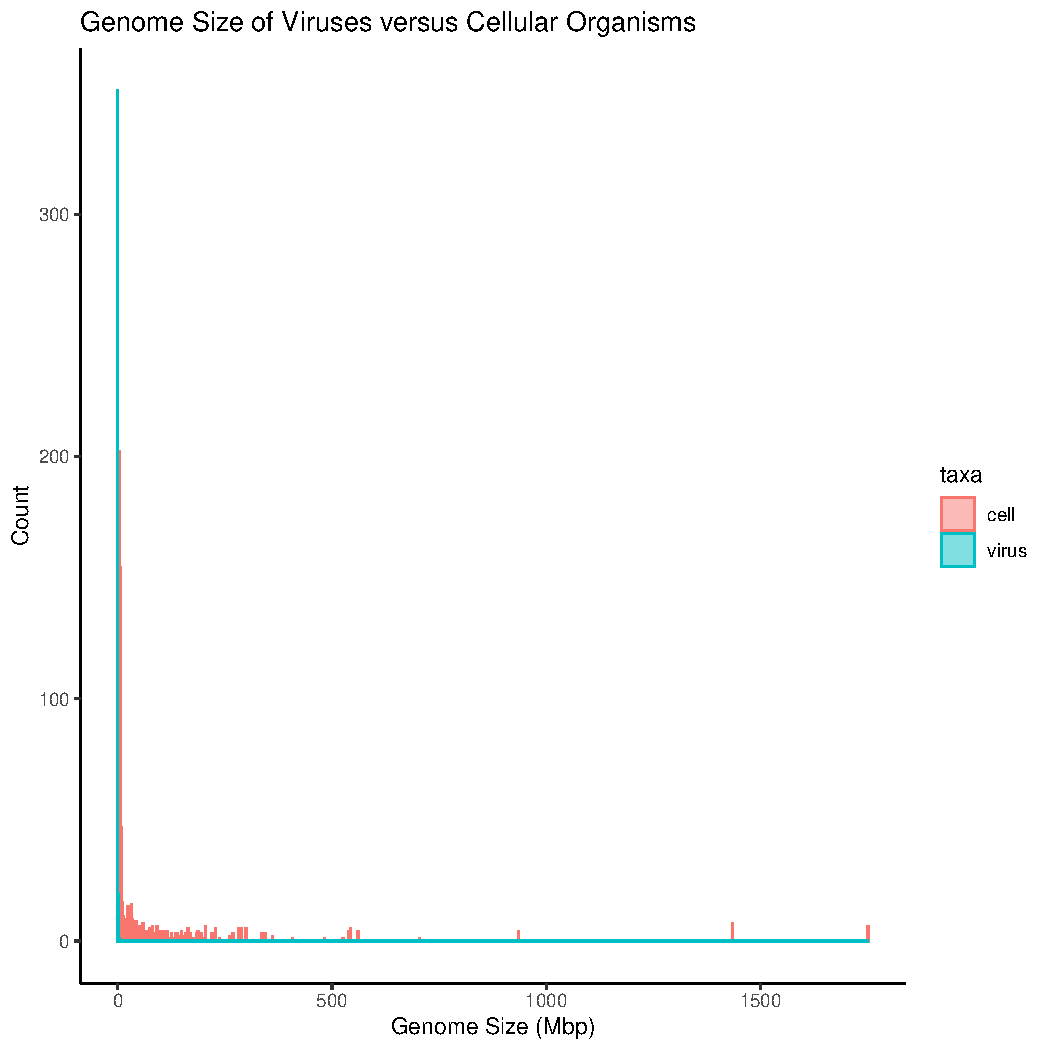
\includegraphics[width=\maxwidth]{figure/unnamed-chunk-2-1} 

\end{knitrout}

Notice that there remain some very large genomes at approxiamtely $1.5$ billion bp. We investigate these large (non-viral) genomes next.
\begin{knitrout}
\definecolor{shadecolor}{rgb}{0.969, 0.969, 0.969}\color{fgcolor}\begin{kframe}
\begin{alltt}
\hlstd{euk} \hlkwb{<-} \hlkwd{induce_tree}\hlstd{(}\hlnum{2759}\hlstd{);}
\hlstd{bac} \hlkwb{<-} \hlkwd{induce_tree}\hlstd{(}\hlnum{2}\hlstd{)}
\hlstd{arch} \hlkwb{<-} \hlkwd{induce_tree}\hlstd{(}\hlnum{2157}\hlstd{)}
\hlstd{cell.hist} \hlkwb{<-} \hlkwd{data.frame}\hlstd{(} \hlkwc{taxa} \hlstd{=} \hlstr{"euk"}\hlstd{,} \hlkwc{genome_size} \hlstd{= euk}\hlopt{$}\hlstd{genome_size[}\hlopt{!}\hlkwd{is.na}\hlstd{(euk}\hlopt{$}\hlstd{genome_size)])}
\hlstd{cell.hist} \hlkwb{<-} \hlkwd{rbind}\hlstd{( cell.hist,} \hlkwd{data.frame}\hlstd{(} \hlkwc{taxa} \hlstd{=} \hlstr{"bac"}\hlstd{,} \hlkwc{genome_size} \hlstd{= bac}\hlopt{$}\hlstd{genome_size[}\hlopt{!}\hlkwd{is.na}\hlstd{(bac}\hlopt{$}\hlstd{genome_size)]))}
\hlstd{cell.hist} \hlkwb{<-} \hlkwd{rbind}\hlstd{( cell.hist,} \hlkwd{data.frame}\hlstd{(} \hlkwc{taxa} \hlstd{=} \hlstr{"arch"}\hlstd{,} \hlkwc{genome_size} \hlstd{= arch}\hlopt{$}\hlstd{genome_size[}\hlopt{!}\hlkwd{is.na}\hlstd{(arch}\hlopt{$}\hlstd{genome_size)]))}
\hlstd{p}\hlkwb{<-}\hlkwd{ggplot}\hlstd{(cell.hist,} \hlkwd{aes}\hlstd{(}\hlkwc{x}\hlstd{=genome_size,} \hlkwc{fill}\hlstd{=taxa,} \hlkwc{color}\hlstd{=taxa))} \hlopt{+}
  \hlkwd{geom_histogram}\hlstd{(}\hlkwc{position}\hlstd{=}\hlstr{"identity"}\hlstd{,} \hlkwc{alpha}\hlstd{=}\hlnum{0.5}\hlstd{,} \hlkwc{binwidth} \hlstd{=} \hlnum{0.1}\hlstd{)} \hlopt{+}
  \hlkwd{labs}\hlstd{(}\hlkwc{title}\hlstd{=}\hlstr{"Genome Size of Cellular Organisms"} \hlstd{,}\hlkwc{x}\hlstd{=}\hlstr{"Genome Size (Mbp)"}\hlstd{,} \hlkwc{y} \hlstd{=} \hlstr{"Count"}\hlstd{)}\hlopt{+}
  \hlkwd{theme_classic}\hlstd{()}
\hlstd{p}
\end{alltt}
\end{kframe}
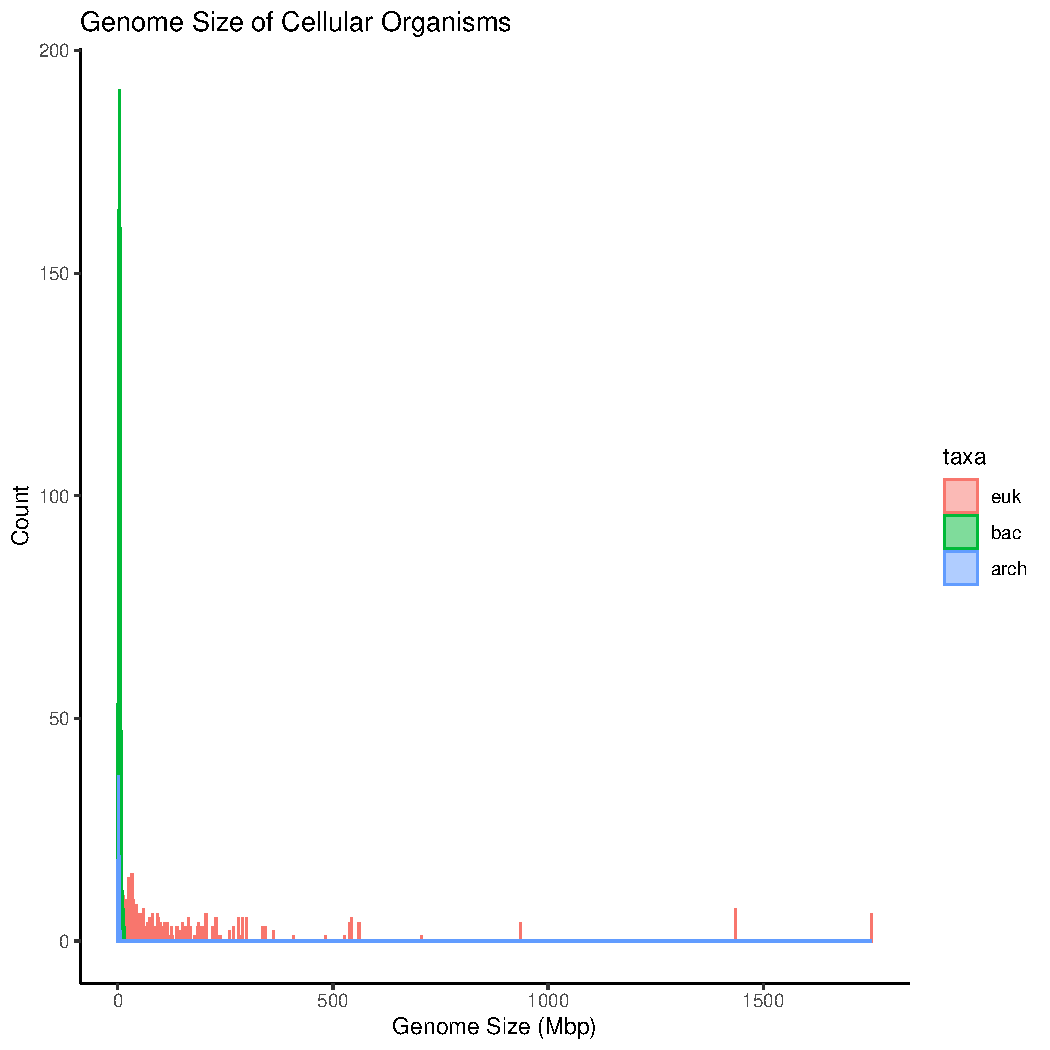
\includegraphics[width=\maxwidth]{figure/unnamed-chunk-3-1} 

\end{knitrout}

The largest bacterial genome in our data is {\em Minicystis rosea} at $16$ Mbp and the largest Archaea genome
is $6$ Mbp.
\begin{knitrout}
\definecolor{shadecolor}{rgb}{0.969, 0.969, 0.969}\color{fgcolor}\begin{kframe}
\begin{alltt}
\hlstd{largest} \hlkwb{<-} \hlkwd{arrange}\hlstd{(bac,}\hlkwd{desc}\hlstd{(genome_size))}
\hlstd{largest_species} \hlkwb{<-} \hlstd{largest[} \hlkwd{which}\hlstd{(largest}\hlopt{$}\hlstd{rank} \hlopt{==} \hlstr{"species"}\hlstd{), ]}

\hlstd{largest} \hlkwb{<-} \hlkwd{arrange}\hlstd{(arch,}\hlkwd{desc}\hlstd{(genome_size))}
\hlstd{largest_species} \hlkwb{<-} \hlstd{largest[} \hlkwd{which}\hlstd{(largest}\hlopt{$}\hlstd{rank} \hlopt{==} \hlstr{"species"}\hlstd{), ]}
\end{alltt}
\end{kframe}
\end{knitrout}

Therefore, we focus our attention on Eukaryota only of which there are many large genomes.

\begin{knitrout}
\definecolor{shadecolor}{rgb}{0.969, 0.969, 0.969}\color{fgcolor}\begin{kframe}
\begin{alltt}
\hlstd{largest} \hlkwb{<-} \hlkwd{arrange}\hlstd{(euk,}\hlkwd{desc}\hlstd{(genome_size))}
\hlstd{largest_species} \hlkwb{<-} \hlstd{largest[} \hlkwd{which}\hlstd{(largest}\hlopt{$}\hlstd{rank} \hlopt{==} \hlstr{"species"}\hlstd{), ]}

\hlstd{p}\hlkwb{<-}\hlkwd{ggplot}\hlstd{(largest,} \hlkwd{aes}\hlstd{(}\hlkwc{x}\hlstd{=genome_size))} \hlopt{+}
  \hlkwd{geom_histogram}\hlstd{(}\hlkwc{position}\hlstd{=}\hlstr{"identity"}\hlstd{,} \hlkwc{alpha}\hlstd{=}\hlnum{0.5}\hlstd{,} \hlkwc{binwidth}\hlstd{=}\hlnum{10}\hlstd{)} \hlopt{+}
  \hlkwd{labs}\hlstd{(}\hlkwc{title}\hlstd{=}\hlstr{"Genome Size of Eukaryota in the Barbadian Reefs"} \hlstd{,}\hlkwc{x}\hlstd{=}\hlstr{"Genome Size (Mbp)"}\hlstd{,} \hlkwc{y} \hlstd{=} \hlstr{"Count"}\hlstd{)}\hlopt{+}
  \hlkwd{theme_classic}\hlstd{()}
\hlstd{p}
\end{alltt}
\end{kframe}
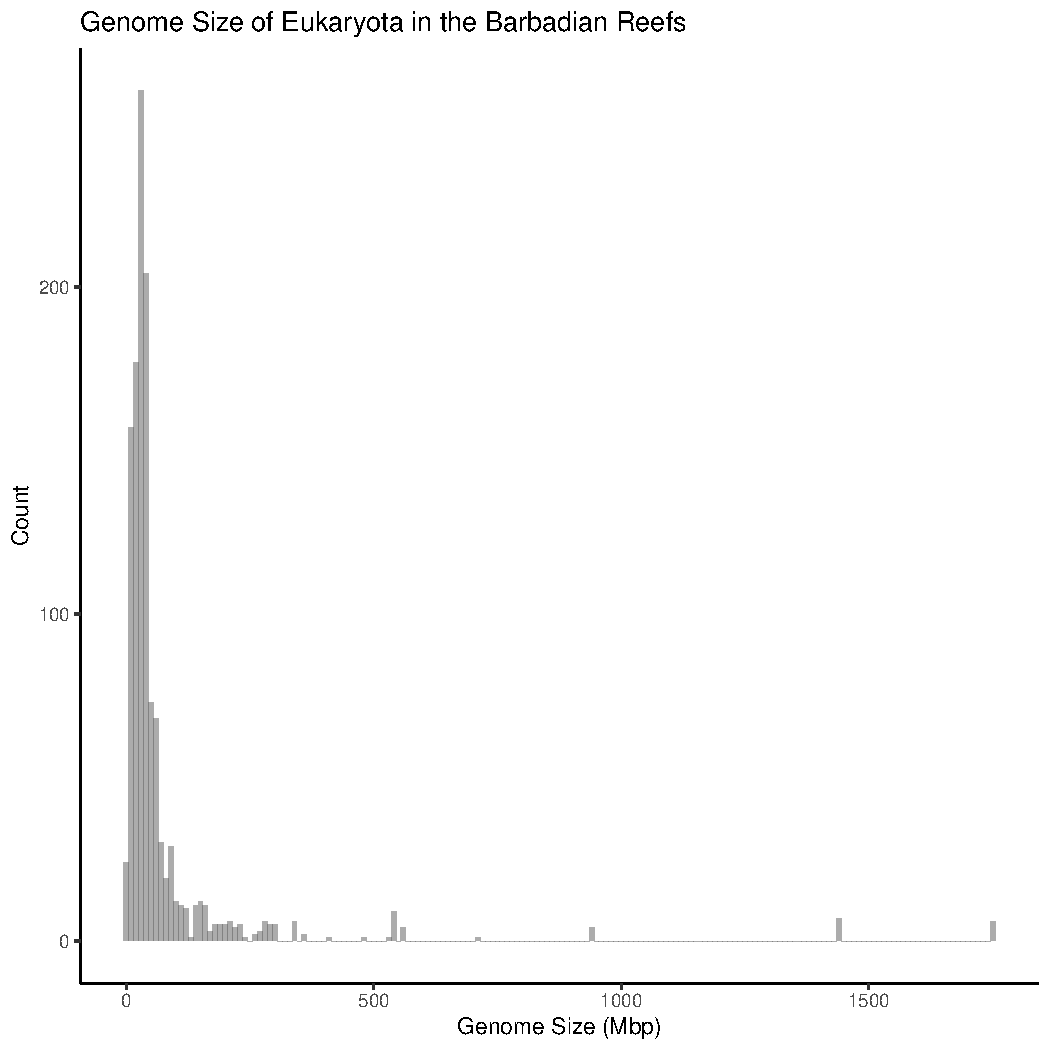
\includegraphics[width=\maxwidth]{figure/unnamed-chunk-5-1} 

\end{knitrout}

Many, but certainly not all, of the large genomes correspond to multicellular organisms. 
We remove the largest ($>30$ Mbp)  from further analysis.
We adjusted the number of counts for each of the remaining genomes that are below this cut off below.

The following taxa were removed.
\begin{knitrout}
\definecolor{shadecolor}{rgb}{0.969, 0.969, 0.969}\color{fgcolor}\begin{kframe}
\begin{alltt}
\hlkwa{for} \hlstd{(i} \hlkwa{in} \hlnum{1}\hlopt{:}\hlnum{200}\hlstd{) \{}
   \hlkwd{cat}\hlstd{(}\hlstr{"\textbackslash{}n"}\hlstd{, largest_species[i,} \hlstr{"name"}\hlstd{],} \hlstr{"\textbackslash{}t\textbackslash{}t"}\hlstd{,  largest_species[i,} \hlstr{"tax_id"}\hlstd{], largest_species[i,} \hlstr{"genome_size"}\hlstd{],} \hlstr{"\textbackslash{}t"}\hlstd{,  largest_species[i,} \hlstr{"path"}\hlstd{] )}
 \hlstd{\}}
\end{alltt}
\begin{verbatim}
## 
##  Chara braunii 		 69332 1751.21 	 root.cellular organisms.Eukaryota.Viridiplantae.Streptophyta.Streptophytina.Charophyceae.Charales.Characeae.Chara.Chara braunii
##  Euglena gracilis 		 3039 1435.5 	 root.cellular organisms.Eukaryota.NA.Euglenozoa.Euglenida.NA.Euglenophyceae.Euglenales.Euglenaceae.Euglena.Euglena gracilis
##  Symbiodinium kawagutii 		 104179 935.067 	 root.cellular organisms.Eukaryota.Sar.Alveolata.Dinophyceae.Suessiales.Symbiodiniaceae.Symbiodinium.Symbiodinium kawagutii
##  Nephromyces sp. ex Molgula occidentalis 		 2544991 560.451 	 root.cellular organisms.Eukaryota.Sar.Alveolata.Apicomplexa.Apicomplexa incertae sedis.Nephromyces.NA.Nephromyces sp. ex Molgula occidentalis
##  Hemileia vastatrix 		 203904 543.605 	 root.cellular organisms.Eukaryota.Opisthokonta.Fungi.Dikarya.Basidiomycota.Pucciniomycotina.Pucciniomycetes.Pucciniales.Pucciniales incertae sedis.Hemileia.Hemileia vastatrix
##  Saccharina japonica 		 88149 539.4045 	 root.cellular organisms.Eukaryota.Sar.Stramenopiles.Ochrophyta.NA.Phaeophyceae.Laminariales.Laminariaceae.Saccharina.Saccharina japonica
##  Dunaliella salina 		 3046 343.704 	 root.cellular organisms.Eukaryota.Viridiplantae.Chlorophyta.core chlorophytes.Chlorophyceae.Chlamydomonadales.Dunaliellaceae.Dunaliella.Dunaliella salina
##  Kappaphycus alvarezii 		 38544 336.721 	 root.cellular organisms.Eukaryota.Rhodophyta.Florideophyceae.NA.Gigartinales.Solieriaceae.Kappaphycus.Kappaphycus alvarezii
##  Digenea simplex 		 945030 299.321 	 root.cellular organisms.Eukaryota.Rhodophyta.Florideophyceae.NA.Ceramiales.Rhodomelaceae.NA.Digenea.Digenea simplex
##  Mesostigma viride 		 41882 289.67 	 root.cellular organisms.Eukaryota.Viridiplantae.Streptophyta.Mesostigmatophyceae.Mesostigmatales.Mesostigmataceae.Mesostigma.Mesostigma viride
##  Cymbomonas tetramitiformis 		 36881 281.27 	 root.cellular organisms.Eukaryota.Viridiplantae.Chlorophyta.Pyramimonadophyceae.Pyramimonadales.NA.Cymbomonas.Cymbomonas tetramitiformis
##  Haematococcus lacustris 		 44745 268.7845 	 root.cellular organisms.Eukaryota.Viridiplantae.Chlorophyta.core chlorophytes.Chlorophyceae.Chlamydomonadales.Haematococcaceae.Haematococcus.Haematococcus lacustris
##  Tetraselmis striata 		 3165 227.954 	 root.cellular organisms.Eukaryota.Viridiplantae.Chlorophyta.core chlorophytes.NA.Chlorodendrales.Chlorodendraceae.Tetraselmis.Tetraselmis striata
##  Oxytricha trifallax 		 1172189 219.9967 	 root.cellular organisms.Eukaryota.Sar.Alveolata.Ciliophora.Intramacronucleata.Spirotrichea.Stichotrichia.NA.Oxytrichidae.Oxytrichinae.Oxytricha.Oxytricha trifallax
##  Physarum polycephalum 		 5791 205.176 	 root.cellular organisms.Eukaryota.NA.NA.Eumycetozoa.Myxogastria.Myxogastromycetidae.Physariida.Physaraceae.Physarum.Physarum polycephalum
##  Ectocarpus siliculosus 		 2880 195.811 	 root.cellular organisms.Eukaryota.Sar.Stramenopiles.Ochrophyta.NA.Phaeophyceae.Ectocarpales.Ectocarpaceae.Ectocarpus.Ectocarpus siliculosus
##  Chromera velia 		 505693 187.455 	 root.cellular organisms.Eukaryota.Sar.Alveolata.Colpodellida.NA.Chromera.Chromera velia
##  Botryococcus braunii 		 38881 184.382 	 root.cellular organisms.Eukaryota.Viridiplantae.Chlorophyta.core chlorophytes.Trebouxiophyceae.Trebouxiophyceae incertae sedis.Elliptochloris clade.Botryococcus.Botryococcus braunii
##  Phytophthora infestans 		 4787 177.7035 	 root.cellular organisms.Eukaryota.Sar.Stramenopiles.Oomycota.Peronosporales.Peronosporaceae.Phytophthora.Phytophthora infestans
##  Cladosiphon okamuranus 		 309737 169.731 	 root.cellular organisms.Eukaryota.Sar.Stramenopiles.Ochrophyta.NA.Phaeophyceae.Ectocarpales.Chordariaceae.Cladosiphon.Cladosiphon okamuranus
##  Trichomonas vaginalis 		 5722 164.072 	 root.cellular organisms.Eukaryota.NA.Parabasalia.Trichomonadida.Trichomonadidae.Trichomonas.Trichomonas vaginalis
##  Cantharellus lutescens 		 104198 160.367 	 root.cellular organisms.Eukaryota.Opisthokonta.Fungi.Dikarya.Basidiomycota.Agaricomycotina.Agaricomycetes.Agaricomycetes incertae sedis.Cantharellales.Cantharellaceae.Cantharellus.Cantharellus lutescens
##  Tetradesmus obliquus 		 3088 157.946 	 root.cellular organisms.Eukaryota.Viridiplantae.Chlorophyta.core chlorophytes.Chlorophyceae.Sphaeropleales.Scenedesmaceae.Tetradesmus.Tetradesmus obliquus
##  NA 		 658196 153.876 	 root.cellular organisms.Eukaryota.Opisthokonta.Fungi.Fungi incertae sedis.Mucoromycota.Glomeromycotina.Glomeromycetes.Glomerales.Glomeraceae.Glomus.NA
##  Gonium pectorale 		 33097 148.806 	 root.cellular organisms.Eukaryota.Viridiplantae.Chlorophyta.core chlorophytes.Chlorophyceae.Chlamydomonadales.Volvocaceae.Gonium.Gonium pectorale
##  NA 		 588596 145.3173 	 root.cellular organisms.Eukaryota.Opisthokonta.Fungi.Fungi incertae sedis.Mucoromycota.Glomeromycotina.Glomeromycetes.Glomerales.Glomeraceae.Rhizophagus.NA
##  Yamagishiella unicocca 		 51707 137.536 	 root.cellular organisms.Eukaryota.Viridiplantae.Chlorophyta.core chlorophytes.Chlorophyceae.Chlamydomonadales.Volvocaceae.Yamagishiella.Yamagishiella unicocca
##  Tetrabaena socialis 		 47790 135.78 	 root.cellular organisms.Eukaryota.Viridiplantae.Chlorophyta.core chlorophytes.Chlorophyceae.Chlamydomonadales.Tetrabaenaceae.Tetrabaena.Tetrabaena socialis
##  Plasmopara halstedii 		 4781 127.0636 	 root.cellular organisms.Eukaryota.Sar.Stramenopiles.Oomycota.Peronosporales.Peronosporaceae.Plasmopara.Plasmopara halstedii
##  Tuber melanosporum 		 39416 124.946 	 root.cellular organisms.Eukaryota.Opisthokonta.Fungi.Dikarya.Ascomycota.saccharomyceta.Pezizomycotina.Pezizomycetes.Pezizales.Tuberaceae.Tuber.Tuber melanosporum
##  Chlamydomonas reinhardtii 		 3055 120.405 	 root.cellular organisms.Eukaryota.Viridiplantae.Chlorophyta.core chlorophytes.Chlorophyceae.Chlamydomonadales.Chlamydomonadaceae.Chlamydomonas.Chlamydomonas reinhardtii
##  Sphaeroforma arctica 		 72019 115.142 	 root.cellular organisms.Eukaryota.Opisthokonta.Ichthyosporea.Ichthyophonida.Sphaeroforma.Sphaeroforma arctica
##  Diplonema papillatum 		 91374 107.915 	 root.cellular organisms.Eukaryota.NA.Euglenozoa.Diplonemea.NA.Diplonema.Diplonema papillatum
##  Pyropia yezoensis 		 2788 107.591 	 root.cellular organisms.Eukaryota.Rhodophyta.Bangiophyceae.Bangiales.Bangiaceae.Pyropia.Pyropia yezoensis
##  Ophiocordyceps sinensis 		 72228 106.603 	 root.cellular organisms.Eukaryota.Opisthokonta.Fungi.Dikarya.Ascomycota.saccharomyceta.Pezizomycotina.leotiomyceta.sordariomyceta.Sordariomycetes.Hypocreomycetidae.Hypocreales.Ophiocordycipitaceae.Ophiocordyceps.Ophiocordyceps sinensis
##  Chondrus crispus 		 2769 104.98 	 root.cellular organisms.Eukaryota.Rhodophyta.Florideophyceae.NA.Gigartinales.Gigartinaceae.Chondrus.Chondrus crispus
##  Cyanophora paradoxa 		 2762 99.9404 	 root.cellular organisms.Eukaryota.Glaucocystophyceae.Cyanophoraceae.Cyanophora.Cyanophora paradoxa
##  Ulva mutabilis 		 498180 98.4847 	 root.cellular organisms.Eukaryota.Viridiplantae.Chlorophyta.Ulvophyceae.OUU clade.Ulvales.Ulvaceae.Ulva.Ulva mutabilis
##  Chlorella sp. ArM0029B 		 1415603 92.9613 	 root.cellular organisms.Eukaryota.Viridiplantae.Chlorophyta.core chlorophytes.Trebouxiophyceae.Chlorellales.Chlorellaceae.Chlorella clade.Chlorella.NA.Chlorella sp. ArM0029B
##  Plasmopara viticola 		 143451 92.59207 	 root.cellular organisms.Eukaryota.Sar.Stramenopiles.Oomycota.Peronosporales.Peronosporaceae.Plasmopara.Plasmopara viticola
##  Thalassiosira oceanica 		 159749 92.1856 	 root.cellular organisms.Eukaryota.Sar.Stramenopiles.Ochrophyta.Bacillariophyta.Coscinodiscophyceae.Thalassiosirophycidae.Thalassiosirales.Thalassiosiraceae.Thalassiosira.Thalassiosira oceanica
##  Psammoneis japonica 		 517775 91.4306 	 root.cellular organisms.Eukaryota.Sar.Stramenopiles.Ochrophyta.Bacillariophyta.NA.Biddulphiophycidae.Triceratiales.Plagiogrammaceae.NA.Psammoneis japonica
##  Ulva prolifera 		 3117 87.8893 	 root.cellular organisms.Eukaryota.Viridiplantae.Chlorophyta.Ulvophyceae.OUU clade.Ulvales.Ulvaceae.Ulva.Ulva prolifera
##  Porphyra umbilicalis 		 2786 87.889 	 root.cellular organisms.Eukaryota.Rhodophyta.Bangiophyceae.Bangiales.Bangiaceae.Porphyra.Porphyra umbilicalis
##  Phytophthora sojae 		 67593 84.23815 	 root.cellular organisms.Eukaryota.Sar.Stramenopiles.Oomycota.Peronosporales.Peronosporaceae.Phytophthora.Phytophthora sojae
##  Acanthamoeba castellanii 		 5755 80.8823 	 root.cellular organisms.Eukaryota.NA.NA.Longamoebia.NA.Acanthamoebidae.Acanthamoeba.Acanthamoeba castellanii
##  Chlamydomonas applanata 		 35704 78.5042 	 root.cellular organisms.Eukaryota.Viridiplantae.Chlorophyta.core chlorophytes.Chlorophyceae.Chlamydomonadales.Chlamydomonadaceae.Chlamydomonas.Chlamydomonas applanata
##  Amanita bisporigera 		 87325 75.3463 	 root.cellular organisms.Eukaryota.Opisthokonta.Fungi.Dikarya.Basidiomycota.Agaricomycotina.Agaricomycetes.Agaricomycetidae.Agaricales.Amanitaceae.Amanita.Amanita bisporigera
##  Chlorokybus atmophyticus 		 3144 74.3303 	 root.cellular organisms.Eukaryota.Viridiplantae.Streptophyta.Chlorokybophyceae.Chlorokybales.Chlorokybaceae.Chlorokybus.Chlorokybus atmophyticus
##  Hyphochytrium catenoides 		 42384 73.08465 	 root.cellular organisms.Eukaryota.Sar.Stramenopiles.Hyphochytriomycetes.Hyphochytriaceae.Hyphochytrium.Hyphochytrium catenoides
##  Hyaloperonospora arabidopsidis 		 272952 72.35685 	 root.cellular organisms.Eukaryota.Sar.Stramenopiles.Oomycota.Peronosporales.Peronosporaceae.Hyaloperonospora.Hyaloperonospora arabidopsidis
##  Paramecium tetraurelia 		 5888 72.0945 	 root.cellular organisms.Eukaryota.Sar.Alveolata.Ciliophora.Intramacronucleata.Oligohymenophorea.Peniculida.Parameciidae.Paramecium.Paramecium tetraurelia
##  Ganoderma boninense 		 34458 69.75715 	 root.cellular organisms.Eukaryota.Opisthokonta.Fungi.Dikarya.Basidiomycota.Agaricomycotina.Agaricomycetes.Agaricomycetes incertae sedis.Polyporales.Polyporaceae.Ganoderma.Ganoderma boninense
##  Monoraphidium neglectum 		 145388 69.7118 	 root.cellular organisms.Eukaryota.Viridiplantae.Chlorophyta.core chlorophytes.Chlorophyceae.Sphaeropleales.Selenastraceae.Monoraphidium.Monoraphidium neglectum
##  Asterionella formosa 		 210441 68.4198 	 root.cellular organisms.Eukaryota.Sar.Stramenopiles.Ochrophyta.Bacillariophyta.Fragilariophyceae.Fragilariophycidae.Fragilariales.Fragilariaceae.Asterionella.Asterionella formosa
##  Sterkiella histriomuscorum 		 94289 66.3686 	 root.cellular organisms.Eukaryota.Sar.Alveolata.Ciliophora.Intramacronucleata.Spirotrichea.Stichotrichia.NA.Oxytrichidae.Stylonychinae.Sterkiella.Sterkiella histriomuscorum
##  Diaporthe helianthi 		 158607 63.672 	 root.cellular organisms.Eukaryota.Opisthokonta.Fungi.Dikarya.Ascomycota.saccharomyceta.Pezizomycotina.leotiomyceta.sordariomyceta.Sordariomycetes.Sordariomycetidae.Diaporthales.Diaporthaceae.Diaporthe.Diaporthe helianthi
##  Rostrostelium ellipticum 		 361140 62.1602 	 root.cellular organisms.Eukaryota.NA.NA.Eumycetozoa.Dictyostelia.Acytosteliales.Acytosteliaceae.Rostrostelium.Rostrostelium ellipticum
##  Aphanomyces invadans 		 157072 61.7834 	 root.cellular organisms.Eukaryota.Sar.Stramenopiles.Oomycota.Saprolegniales.Saprolegniaceae.Aphanomyces.Aphanomyces invadans
##  Toxoplasma gondii 		 5811 61.5763 	 root.cellular organisms.Eukaryota.Sar.Alveolata.Apicomplexa.Conoidasida.Coccidia.Eucoccidiorida.Eimeriorina.Sarcocystidae.Toxoplasma.Toxoplasma gondii
##  NA 		 554055 61.0189 	 root.cellular organisms.Eukaryota.Viridiplantae.Chlorophyta.core chlorophytes.Trebouxiophyceae.Chlorellales.Chlorellaceae.Chlorella clade.Micractinium.NA
##  Eimeria mitis 		 44415 60.4151 	 root.cellular organisms.Eukaryota.Sar.Alveolata.Apicomplexa.Conoidasida.Coccidia.Eucoccidiorida.Eimeriorina.Eimeriidae.Eimeria.Eimeria mitis
##  Armillaria ostoyae 		 47428 60.1068 	 root.cellular organisms.Eukaryota.Opisthokonta.Fungi.Dikarya.Basidiomycota.Agaricomycotina.Agaricomycetes.Agaricomycetidae.Agaricales.Physalacriaceae.Armillaria.Armillaria ostoyae
##  Colletotrichum graminicola 		 31870 59.9141 	 root.cellular organisms.Eukaryota.Opisthokonta.Fungi.Dikarya.Ascomycota.saccharomyceta.Pezizomycotina.leotiomyceta.sordariomyceta.Sordariomycetes.Hypocreomycetidae.Glomerellales.NA.Colletotrichum.Colletotrichum graminicola species complex.Colletotrichum graminicola
##  Aphanomyces astaci 		 112090 59.69445 	 root.cellular organisms.Eukaryota.Sar.Stramenopiles.Oomycota.Saprolegniales.Saprolegniaceae.Aphanomyces.Aphanomyces astaci
##  Phytophthora cinnamomi 		 4785 59.63075 	 root.cellular organisms.Eukaryota.Sar.Stramenopiles.Oomycota.Peronosporales.Peronosporaceae.Phytophthora.Phytophthora cinnamomi
##  Parachlorella kessleri 		 3074 59.1878 	 root.cellular organisms.Eukaryota.Viridiplantae.Chlorophyta.core chlorophytes.Trebouxiophyceae.Chlorellales.Chlorellaceae.Parachlorella.Parachlorella kessleri
##  Chrysochromulina tobinii 		 1460289 59.0731 	 root.cellular organisms.Eukaryota.NA.Haptophyta.NA.Prymnesiales.Chrysochromulinaceae.Chrysochromulina.Chrysochromulina tobinii
##  Besnoitia besnoiti 		 94643 58.8459 	 root.cellular organisms.Eukaryota.Sar.Alveolata.Apicomplexa.Conoidasida.Coccidia.Eucoccidiorida.Eimeriorina.Sarcocystidae.Besnoitia.Besnoitia besnoiti
##  Moneuplotes crassus 		 5936 58.5666 	 root.cellular organisms.Eukaryota.Sar.Alveolata.Ciliophora.Intramacronucleata.Spirotrichea.Hypotrichia.Euplotida.Euplotidae.Moneuplotes.Moneuplotes crassus
##  Chlorella sorokiniana 		 3076 58.33862 	 root.cellular organisms.Eukaryota.Viridiplantae.Chlorophyta.core chlorophytes.Trebouxiophyceae.Chlorellales.Chlorellaceae.Chlorella clade.Chlorella.Chlorella sorokiniana
##  NA 		 690256 57.55417 	 root.cellular organisms.Eukaryota.Opisthokonta.Fungi.Dikarya.Ascomycota.saccharomyceta.Pezizomycotina.leotiomyceta.sordariomyceta.Sordariomycetes.Hypocreomycetidae.Glomerellales.NA.Colletotrichum.Colletotrichum gloeosporioides species complex.NA
##  Mastigamoeba balamuthi 		 108607 57.2666 	 root.cellular organisms.Eukaryota.NA.NA.NA.NA.Mastigamoebidae.Mastigamoeba.Mastigamoeba balamuthi
##  Colletotrichum gloeosporioides 		 474922 57.2517 	 root.cellular organisms.Eukaryota.Opisthokonta.Fungi.Dikarya.Ascomycota.saccharomyceta.Pezizomycotina.leotiomyceta.sordariomyceta.Sordariomycetes.Hypocreomycetidae.Glomerellales.NA.Colletotrichum.Colletotrichum gloeosporioides species complex.Colletotrichum gloeosporioides
##  Auxenochlorella pyrenoidosa 		 3078 56.993 	 root.cellular organisms.Eukaryota.Viridiplantae.Chlorophyta.core chlorophytes.Trebouxiophyceae.Chlorellales.Chlorellaceae.Auxenochlorella.Auxenochlorella pyrenoidosa
##  Aphanomyces euteiches 		 100861 56.9046 	 root.cellular organisms.Eukaryota.Sar.Stramenopiles.Oomycota.Saprolegniales.Saprolegniaceae.Aphanomyces.Aphanomyces euteiches
##  Aureococcus anophagefferens 		 44056 56.6606 	 root.cellular organisms.Eukaryota.Sar.Stramenopiles.Pelagophyceae.Pelagomonadales.Aureococcus.Aureococcus anophagefferens
##  Rhizoctonia solani 		 456999 56.0285 	 root.cellular organisms.Eukaryota.Opisthokonta.Fungi.Dikarya.Basidiomycota.Agaricomycotina.Agaricomycetes.Agaricomycetes incertae sedis.Cantharellales.Ceratobasidiaceae.Rhizoctonia.Rhizoctonia solani
##  Salpingoeca rosetta 		 946362 55.4403 	 root.cellular organisms.Eukaryota.Opisthokonta.Choanoflagellata.Craspedida.Salpingoecidae.Salpingoeca.Salpingoeca rosetta
##  Clonostachys rosea 		 29856 55.30035 	 root.cellular organisms.Eukaryota.Opisthokonta.Fungi.Dikarya.Ascomycota.saccharomyceta.Pezizomycotina.leotiomyceta.sordariomyceta.Sordariomycetes.Hypocreomycetidae.Hypocreales.Bionectriaceae.Clonostachys.Clonostachys rosea
##  Eimeria necatrix 		 51315 55.0079 	 root.cellular organisms.Eukaryota.Sar.Alveolata.Apicomplexa.Conoidasida.Coccidia.Eucoccidiorida.Eimeriorina.Eimeriidae.Eimeria.Eimeria necatrix
##  Amorphotheca resinae 		 5101 54.4745 	 root.cellular organisms.Eukaryota.Opisthokonta.Fungi.Dikarya.Ascomycota.saccharomyceta.Pezizomycotina.leotiomyceta.sordariomyceta.Leotiomycetes.Leotiomycetes incertae sedis.Myxotrichaceae.Amorphotheca.Amorphotheca resinae
##  Phytophthora capsici 		 4784 53.41358 	 root.cellular organisms.Eukaryota.Sar.Stramenopiles.Oomycota.Peronosporales.Peronosporaceae.Phytophthora.Phytophthora capsici
##  Porodaedalea pini 		 108901 53.3469 	 root.cellular organisms.Eukaryota.Opisthokonta.Fungi.Dikarya.Basidiomycota.Agaricomycotina.Agaricomycetes.Agaricomycetes incertae sedis.Hymenochaetales.Hymenochaetaceae.Porodaedalea.Porodaedalea pini
##  Pyropia haitanensis 		 1262161 53.2546 	 root.cellular organisms.Eukaryota.Rhodophyta.Bangiophyceae.Bangiales.Bangiaceae.Pyropia.Pyropia haitanensis
##  Fusarium oxysporum 		 5507 52.02895 	 root.cellular organisms.Eukaryota.Opisthokonta.Fungi.Dikarya.Ascomycota.saccharomyceta.Pezizomycotina.leotiomyceta.sordariomyceta.Sordariomycetes.Hypocreomycetidae.Hypocreales.Nectriaceae.Fusarium.Fusarium oxysporum species complex.Fusarium oxysporum
##  Stichococcus bacillaris 		 37433 51.9927 	 root.cellular organisms.Eukaryota.Viridiplantae.Chlorophyta.core chlorophytes.Trebouxiophyceae.Prasiolales.Prasiolaceae.Stichococcus.Stichococcus bacillaris
##  Raphidocelis subcapitata 		 307507 51.1627 	 root.cellular organisms.Eukaryota.Viridiplantae.Chlorophyta.core chlorophytes.Chlorophyceae.Sphaeropleales.Selenastraceae.Raphidocelis.Raphidocelis subcapitata
##  Stylonychia lemnae 		 5949 50.1645 	 root.cellular organisms.Eukaryota.Sar.Alveolata.Ciliophora.Intramacronucleata.Spirotrichea.Stichotrichia.NA.Oxytrichidae.Stylonychinae.Stylonychia.Stylonychia lemnae
##  Morchella importuna 		 1174673 49.9687 	 root.cellular organisms.Eukaryota.Opisthokonta.Fungi.Dikarya.Ascomycota.saccharomyceta.Pezizomycotina.Pezizomycetes.Pezizales.Morchellaceae.Morchella.Morchella elata clade.Morchella importuna
##  Fistulifera solaris 		 1519565 49.7366 	 root.cellular organisms.Eukaryota.Sar.Stramenopiles.Ochrophyta.Bacillariophyta.Bacillariophyceae.Bacillariophycidae.Naviculales.Naviculaceae.Fistulifera.Fistulifera solaris
##  Colletotrichum higginsianum 		 80884 49.4357 	 root.cellular organisms.Eukaryota.Opisthokonta.Fungi.Dikarya.Ascomycota.saccharomyceta.Pezizomycotina.leotiomyceta.sordariomyceta.Sordariomycetes.Hypocreomycetidae.Glomerellales.NA.Colletotrichum.Colletotrichum destructivum species complex.Colletotrichum higginsianum
##  Phialocephala scopiformis 		 149040 48.8763 	 root.cellular organisms.Eukaryota.Opisthokonta.Fungi.Dikarya.Ascomycota.saccharomyceta.Pezizomycotina.leotiomyceta.sordariomyceta.Leotiomycetes.Helotiales.Helotiales incertae sedis.Phialocephala.Phialocephala scopiformis
##  Ichthyophthirius multifiliis 		 5932 48.8 	 root.cellular organisms.Eukaryota.Sar.Alveolata.Ciliophora.Intramacronucleata.Oligohymenophorea.Hymenostomatida.Ophryoglenina.Ichthyophthirius.Ichthyophthirius multifiliis
##  Coremiostelium polycephalum 		 142831 48.621 	 root.cellular organisms.Eukaryota.NA.NA.Eumycetozoa.Dictyostelia.Dictyosteliales.Coremiostelium.Coremiostelium polycephalum
##  Colletotrichum orchidophilum 		 1209926 48.5565 	 root.cellular organisms.Eukaryota.Opisthokonta.Fungi.Dikarya.Ascomycota.saccharomyceta.Pezizomycotina.leotiomyceta.sordariomyceta.Sordariomycetes.Hypocreomycetidae.Glomerellales.NA.Colletotrichum.Colletotrichum orchidophilum
##  NA 		 1578925 48.3379 	 root.cellular organisms.Eukaryota.Opisthokonta.Fungi.Dikarya.Ascomycota.saccharomyceta.Pezizomycotina.leotiomyceta.sordariomyceta.Sordariomycetes.Sordariomycetidae.NA.Pyriculariaceae.Pyricularia.NA
##  Phytophthora parasitica 		 4792 47.7626 	 root.cellular organisms.Eukaryota.Sar.Stramenopiles.Oomycota.Peronosporales.Peronosporaceae.Phytophthora.Phytophthora parasitica
##  NA 		 554065 46.1595 	 root.cellular organisms.Eukaryota.Viridiplantae.Chlorophyta.core chlorophytes.Trebouxiophyceae.Chlorellales.Chlorellaceae.Chlorella clade.Chlorella.NA
##  Leptosphaeria maculans 		 5022 45.9865 	 root.cellular organisms.Eukaryota.Opisthokonta.Fungi.Dikarya.Ascomycota.saccharomyceta.Pezizomycotina.leotiomyceta.dothideomyceta.Dothideomycetes.Pleosporomycetidae.Pleosporales.Pleosporineae.Leptosphaeriaceae.Leptosphaeria.Leptosphaeria maculans species complex.Leptosphaeria maculans
##  Eimeria maxima 		 5804 45.9751 	 root.cellular organisms.Eukaryota.Sar.Alveolata.Apicomplexa.Conoidasida.Coccidia.Eucoccidiorida.Eimeriorina.Eimeriidae.Eimeria.Eimeria maxima
##  Eimeria acervulina 		 5801 45.8306 	 root.cellular organisms.Eukaryota.Sar.Alveolata.Apicomplexa.Conoidasida.Coccidia.Eucoccidiorida.Eimeriorina.Eimeriidae.Eimeria.Eimeria acervulina
##  Trichoderma virens 		 29875 45.8201 	 root.cellular organisms.Eukaryota.Opisthokonta.Fungi.Dikarya.Ascomycota.saccharomyceta.Pezizomycotina.leotiomyceta.sordariomyceta.Sordariomycetes.Hypocreomycetidae.Hypocreales.Hypocreaceae.Trichoderma.Trichoderma virens
##  Fusarium solani 		 169388 45.8133 	 root.cellular organisms.Eukaryota.Opisthokonta.Fungi.Dikarya.Ascomycota.saccharomyceta.Pezizomycotina.leotiomyceta.sordariomyceta.Sordariomycetes.Hypocreomycetidae.Hypocreales.Nectriaceae.Fusarium.Fusarium solani species complex.Fusarium solani
##  Fusarium proliferatum 		 948311 45.78918 	 root.cellular organisms.Eukaryota.Opisthokonta.Fungi.Dikarya.Ascomycota.saccharomyceta.Pezizomycotina.leotiomyceta.sordariomyceta.Sordariomycetes.Hypocreomycetidae.Hypocreales.Nectriaceae.Fusarium.Fusarium fujikuroi species complex.Fusarium proliferatum
##  Aspergillus mulundensis 		 1810919 45.3419 	 root.cellular organisms.Eukaryota.Opisthokonta.Fungi.Dikarya.Ascomycota.saccharomyceta.Pezizomycotina.leotiomyceta.Eurotiomycetes.Eurotiomycetidae.Eurotiales.Aspergillaceae.Aspergillus.Aspergillus mulundensis
##  Rhizopus oryzae 		 64495 45.04514 	 root.cellular organisms.Eukaryota.Opisthokonta.Fungi.Fungi incertae sedis.Mucoromycota.Mucoromycotina.Mucoromycetes.Mucorales.Mucorineae.Rhizopodaceae.Rhizopus.Rhizopus oryzae
##  Fusarium fujikuroi 		 5127 44.92106 	 root.cellular organisms.Eukaryota.Opisthokonta.Fungi.Dikarya.Ascomycota.saccharomyceta.Pezizomycotina.leotiomyceta.sordariomyceta.Sordariomycetes.Hypocreomycetidae.Hypocreales.Nectriaceae.Fusarium.Fusarium fujikuroi species complex.Fusarium fujikuroi
##  Agrocybe aegerita 		 5400 44.7908 	 root.cellular organisms.Eukaryota.Opisthokonta.Fungi.Dikarya.Basidiomycota.Agaricomycotina.Agaricomycetes.Agaricomycetidae.Agaricales.Bolbitiaceae.Agrocybe.Agrocybe aegerita
##  Chrysoporthe austroafricana 		 354353 44.6689 	 root.cellular organisms.Eukaryota.Opisthokonta.Fungi.Dikarya.Ascomycota.saccharomyceta.Pezizomycotina.leotiomyceta.sordariomyceta.Sordariomycetes.Sordariomycetidae.Diaporthales.Cryphonectriaceae.Cryphonectria-Endothia species complex.Chrysoporthe.Chrysoporthe austroafricana
##  Pyricularia grisea 		 148305 44.31875 	 root.cellular organisms.Eukaryota.Opisthokonta.Fungi.Dikarya.Ascomycota.saccharomyceta.Pezizomycotina.leotiomyceta.sordariomyceta.Sordariomycetes.Sordariomycetidae.NA.Pyriculariaceae.Pyricularia.Pyricularia grisea
##  Pseudocercospora fijiensis 		 1873960 44.1245 	 root.cellular organisms.Eukaryota.Opisthokonta.Fungi.Dikarya.Ascomycota.saccharomyceta.Pezizomycotina.leotiomyceta.dothideomyceta.Dothideomycetes.Dothideomycetidae.Capnodiales.Mycosphaerellaceae.Pseudocercospora.Pseudocercospora fijiensis
##  Pythium insidiosum 		 114742 44.08819 	 root.cellular organisms.Eukaryota.Sar.Stramenopiles.Oomycota.Pythiales.Pythiaceae.Pythium.Pythium insidiosum
##  Cyclospora cayetanensis 		 88456 43.98724 	 root.cellular organisms.Eukaryota.Sar.Alveolata.Apicomplexa.Conoidasida.Coccidia.Eucoccidiorida.Eimeriorina.Eimeriidae.Cyclospora.Cyclospora cayetanensis
##  NA 		 563466 43.82915 	 root.cellular organisms.Eukaryota.Opisthokonta.Fungi.Dikarya.Ascomycota.saccharomyceta.Pezizomycotina.leotiomyceta.sordariomyceta.Sordariomycetes.Hypocreomycetidae.Microascales.Microascaceae.Scedosporium.NA
##  Eimeria falciformis 		 84963 43.6713 	 root.cellular organisms.Eukaryota.Sar.Alveolata.Apicomplexa.Conoidasida.Coccidia.Eucoccidiorida.Eimeriorina.Eimeriidae.Eimeria.Eimeria falciformis
##  Achlya hypogyna 		 1202772 43.3985 	 root.cellular organisms.Eukaryota.Sar.Stramenopiles.Oomycota.Saprolegniales.Saprolegniaceae.Achlya.Achlya hypogyna
##  Venturia effusa 		 50376 42.9507 	 root.cellular organisms.Eukaryota.Opisthokonta.Fungi.Dikarya.Ascomycota.saccharomyceta.Pezizomycotina.leotiomyceta.dothideomyceta.Dothideomycetes.Pleosporomycetidae.Venturiales.Venturiaceae.Venturia.Venturia effusa
##  Lobosporangium transversale 		 64571 42.7689 	 root.cellular organisms.Eukaryota.Opisthokonta.Fungi.Fungi incertae sedis.Mucoromycota.Mortierellomycotina.Mortierellomycetes.Mortierellales.Mortierellaceae.Lobosporangium.Lobosporangium transversale
##  [Nectria] haematococca 		 140110 42.65957 	 root.cellular organisms.Eukaryota.Opisthokonta.Fungi.Dikarya.Ascomycota.saccharomyceta.Pezizomycotina.leotiomyceta.sordariomyceta.Sordariomycetes.Hypocreomycetidae.Hypocreales.Nectriaceae.Fusarium.Fusarium solani species complex.[Nectria] haematococca
##  Fusarium verticillioides 		 117187 42.40943 	 root.cellular organisms.Eukaryota.Opisthokonta.Fungi.Dikarya.Ascomycota.saccharomyceta.Pezizomycotina.leotiomyceta.sordariomyceta.Sordariomycetes.Hypocreomycetidae.Hypocreales.Nectriaceae.Fusarium.Fusarium fujikuroi species complex.Fusarium verticillioides
##  Trichosporon coremiiforme 		 82509 42.3533 	 root.cellular organisms.Eukaryota.Opisthokonta.Fungi.Dikarya.Basidiomycota.Agaricomycotina.Tremellomycetes.Trichosporonales.NA.Trichosporon.Trichosporon coremiiforme
##  NA 		 569365 42.30655 	 root.cellular organisms.Eukaryota.Opisthokonta.Fungi.Dikarya.Ascomycota.saccharomyceta.Pezizomycotina.leotiomyceta.Eurotiomycetes.Chaetothyriomycetidae.Chaetothyriales.Herpotrichiellaceae.Cladophialophora.NA
##  Lentinula edodes 		 5353 41.46406 	 root.cellular organisms.Eukaryota.Opisthokonta.Fungi.Dikarya.Basidiomycota.Agaricomycotina.Agaricomycetes.Agaricomycetidae.Agaricales.Omphalotaceae.Lentinula.Lentinula edodes
##  Crithidia fasciculata 		 5656 41.2974 	 root.cellular organisms.Eukaryota.NA.Euglenozoa.Kinetoplastea.Metakinetoplastina.Trypanosomatida.Trypanosomatidae.Leishmaniinae.Crithidia.Crithidia fasciculata
##  Trypanosoma congolense 		 5692 41.2334 	 root.cellular organisms.Eukaryota.NA.Euglenozoa.Kinetoplastea.Metakinetoplastina.Trypanosomatida.Trypanosomatidae.Trypanosoma.Nannomonas.Trypanosoma congolense
##  Annulohypoxylon stygium 		 326628 41.1319 	 root.cellular organisms.Eukaryota.Opisthokonta.Fungi.Dikarya.Ascomycota.saccharomyceta.Pezizomycotina.leotiomyceta.sordariomyceta.Sordariomycetes.Xylariomycetidae.Xylariales.NA.Annulohypoxylon.Annulohypoxylon stygium
##  Chlorella vulgaris 		 3077 41.10782 	 root.cellular organisms.Eukaryota.Viridiplantae.Chlorophyta.core chlorophytes.Trebouxiophyceae.Chlorellales.Chlorellaceae.Chlorella clade.Chlorella.Chlorella vulgaris
##  Neurospora crassa 		 5141 40.98185 	 root.cellular organisms.Eukaryota.Opisthokonta.Fungi.Dikarya.Ascomycota.saccharomyceta.Pezizomycotina.leotiomyceta.sordariomyceta.Sordariomycetes.Sordariomycetidae.Sordariales.Sordariaceae.Neurospora.Neurospora crassa
##  Naegleria gruberi 		 5762 40.9641 	 root.cellular organisms.Eukaryota.NA.Heterolobosea.NA.NA.Vahlkampfiidae.Naegleria.Naegleria gruberi
##  Trichosporon ovoides 		 82524 40.9337 	 root.cellular organisms.Eukaryota.Opisthokonta.Fungi.Dikarya.Basidiomycota.Agaricomycotina.Tremellomycetes.Trichosporonales.NA.Trichosporon.Trichosporon ovoides
##  Phialemoniopsis curvata 		 1093900 40.3666 	 root.cellular organisms.Eukaryota.Opisthokonta.Fungi.Dikarya.Ascomycota.saccharomyceta.Pezizomycotina.leotiomyceta.sordariomyceta.Sordariomycetes.Xylariomycetidae.Xylariales.Xylariales incertae sedis.Phialemoniopsis.Phialemoniopsis curvata
##  NA 		 568076 40.3173 	 root.cellular organisms.Eukaryota.Opisthokonta.Fungi.Dikarya.Ascomycota.saccharomyceta.Pezizomycotina.leotiomyceta.sordariomyceta.Sordariomycetes.Hypocreomycetidae.Hypocreales.Clavicipitaceae.Metarhizium.NA
##  Trichoderma harzianum 		 5544 40.25984 	 root.cellular organisms.Eukaryota.Opisthokonta.Fungi.Dikarya.Ascomycota.saccharomyceta.Pezizomycotina.leotiomyceta.sordariomyceta.Sordariomycetes.Hypocreomycetidae.Hypocreales.Hypocreaceae.Trichoderma.Trichoderma harzianum
##  Aspergillus alliaceus 		 209559 40.15425 	 root.cellular organisms.Eukaryota.Opisthokonta.Fungi.Dikarya.Ascomycota.saccharomyceta.Pezizomycotina.leotiomyceta.Eurotiomycetes.Eurotiomycetidae.Eurotiales.Aspergillaceae.Aspergillus.Aspergillus alliaceus
##  Aspergillus sojae 		 41058 40.054 	 root.cellular organisms.Eukaryota.Opisthokonta.Fungi.Dikarya.Ascomycota.saccharomyceta.Pezizomycotina.leotiomyceta.Eurotiomycetes.Eurotiomycetidae.Eurotiales.Aspergillaceae.Aspergillus.Aspergillus sojae
##  Fusarium culmorum 		 5516 40.0196 	 root.cellular organisms.Eukaryota.Opisthokonta.Fungi.Dikarya.Ascomycota.saccharomyceta.Pezizomycotina.leotiomyceta.sordariomyceta.Sordariomycetes.Hypocreomycetidae.Hypocreales.Nectriaceae.Fusarium.NA.Fusarium culmorum
##  Aspergillus caelatus 		 61420 40.0164 	 root.cellular organisms.Eukaryota.Opisthokonta.Fungi.Dikarya.Ascomycota.saccharomyceta.Pezizomycotina.leotiomyceta.Eurotiomycetes.Eurotiomycetidae.Eurotiales.Aspergillaceae.Aspergillus.Aspergillus caelatus
##  Arthrobotrys oligospora 		 13349 40.00234 	 root.cellular organisms.Eukaryota.Opisthokonta.Fungi.Dikarya.Ascomycota.saccharomyceta.Pezizomycotina.Orbiliomycetes.Orbiliales.Orbiliaceae.Arthrobotrys.Arthrobotrys oligospora
##  Bodo saltans 		 75058 39.8644 	 root.cellular organisms.Eukaryota.NA.Euglenozoa.Kinetoplastea.Metakinetoplastina.Eubodonida.Bodonidae.Bodo.Bodo saltans
##  Schizophyllum commune 		 5334 39.7789 	 root.cellular organisms.Eukaryota.Opisthokonta.Fungi.Dikarya.Basidiomycota.Agaricomycotina.Agaricomycetes.Agaricomycetidae.Agaricales.Schizophyllaceae.Schizophyllum.Schizophyllum commune
##  Hypoxylon pulicicidum 		 1243767 39.6241 	 root.cellular organisms.Eukaryota.Opisthokonta.Fungi.Dikarya.Ascomycota.saccharomyceta.Pezizomycotina.leotiomyceta.sordariomyceta.Sordariomycetes.Xylariomycetidae.Xylariales.NA.Hypoxylon.Hypoxylon pulicicidum
##  Pyricularia oryzae 		 318829 39.4074 	 root.cellular organisms.Eukaryota.Opisthokonta.Fungi.Dikarya.Ascomycota.saccharomyceta.Pezizomycotina.leotiomyceta.sordariomyceta.Sordariomycetes.Sordariomycetidae.NA.Pyriculariaceae.Pyricularia.Pyricularia oryzae
##  Cryphonectria parasitica 		 5116 39.2611 	 root.cellular organisms.Eukaryota.Opisthokonta.Fungi.Dikarya.Ascomycota.saccharomyceta.Pezizomycotina.leotiomyceta.sordariomyceta.Sordariomycetes.Sordariomycetidae.Diaporthales.Cryphonectriaceae.Cryphonectria-Endothia species complex.Cryphonectria.Cryphonectria parasitica
##  Phanerochaete chrysosporium 		 5306 39.2051 	 root.cellular organisms.Eukaryota.Opisthokonta.Fungi.Dikarya.Basidiomycota.Agaricomycotina.Agaricomycetes.Agaricomycetes incertae sedis.Polyporales.Phanerochaetaceae.Phanerochaete.Phanerochaete chrysosporium
##  Thraustotheca clavata 		 74557 39.1007 	 root.cellular organisms.Eukaryota.Sar.Stramenopiles.Oomycota.Saprolegniales.Saprolegniaceae.Thraustotheca.Thraustotheca clavata
##  Sparassis crispa 		 139825 39.0203 	 root.cellular organisms.Eukaryota.Opisthokonta.Fungi.Dikarya.Basidiomycota.Agaricomycotina.Agaricomycetes.Agaricomycetes incertae sedis.Polyporales.Sparassidaceae.Sparassis.Sparassis crispa
##  Sordaria macrospora 		 5147 38.8634 	 root.cellular organisms.Eukaryota.Opisthokonta.Fungi.Dikarya.Ascomycota.saccharomyceta.Pezizomycotina.leotiomyceta.sordariomyceta.Sordariomycetes.Sordariomycetidae.Sordariales.Sordariaceae.Sordaria.Sordaria macrospora
##  Fusarium venenatum 		 56646 38.6602 	 root.cellular organisms.Eukaryota.Opisthokonta.Fungi.Dikarya.Ascomycota.saccharomyceta.Pezizomycotina.leotiomyceta.sordariomyceta.Sordariomycetes.Hypocreomycetidae.Hypocreales.Nectriaceae.Fusarium.NA.Fusarium venenatum
##  Dichomitus squalens 		 114155 38.59503 	 root.cellular organisms.Eukaryota.Opisthokonta.Fungi.Dikarya.Basidiomycota.Agaricomycotina.Agaricomycetes.Agaricomycetes incertae sedis.Polyporales.Polyporaceae.Dichomitus.Dichomitus squalens
##  NA 		 1725355 38.5165 	 root.cellular organisms.Eukaryota.Opisthokonta.Fungi.Dikarya.Ascomycota.saccharomyceta.Saccharomycotina.Saccharomycetes.Saccharomycetales.Saccharomycopsidaceae.Saccharomycopsis.NA
##  Paraphaeosphaeria sporulosa 		 1460663 38.464 	 root.cellular organisms.Eukaryota.Opisthokonta.Fungi.Dikarya.Ascomycota.saccharomyceta.Pezizomycotina.leotiomyceta.dothideomyceta.Dothideomycetes.Pleosporomycetidae.Pleosporales.Massarineae.Didymosphaeriaceae.Paraphaeosphaeria.Paraphaeosphaeria sporulosa
##  Aspergillus pseudotamarii 		 132259 38.2439 	 root.cellular organisms.Eukaryota.Opisthokonta.Fungi.Dikarya.Ascomycota.saccharomyceta.Pezizomycotina.leotiomyceta.Eurotiomycetes.Eurotiomycetidae.Eurotiales.Aspergillaceae.Aspergillus.Aspergillus pseudotamarii
##  Exophiala oligosperma 		 215243 38.2245 	 root.cellular organisms.Eukaryota.Opisthokonta.Fungi.Dikarya.Ascomycota.saccharomyceta.Pezizomycotina.leotiomyceta.Eurotiomycetes.Chaetothyriomycetidae.Chaetothyriales.Herpotrichiellaceae.Exophiala.Exophiala oligosperma
##  Trichoderma gamsii 		 398673 38.1993 	 root.cellular organisms.Eukaryota.Opisthokonta.Fungi.Dikarya.Ascomycota.saccharomyceta.Pezizomycotina.leotiomyceta.sordariomyceta.Sordariomycetes.Hypocreomycetidae.Hypocreales.Hypocreaceae.Trichoderma.Trichoderma gamsii
##  Zymoseptoria tritici 		 1047171 38.1077 	 root.cellular organisms.Eukaryota.Opisthokonta.Fungi.Dikarya.Ascomycota.saccharomyceta.Pezizomycotina.leotiomyceta.dothideomyceta.Dothideomycetes.Dothideomycetidae.Capnodiales.Mycosphaerellaceae.Zymoseptoria.Zymoseptoria tritici
##  Trichoderma asperellum 		 101201 38.0794 	 root.cellular organisms.Eukaryota.Opisthokonta.Fungi.Dikarya.Ascomycota.saccharomyceta.Pezizomycotina.leotiomyceta.sordariomyceta.Sordariomycetes.Hypocreomycetidae.Hypocreales.Hypocreaceae.Trichoderma.Trichoderma asperellum
##  Parastagonospora nodorum 		 13684 38.03676 	 root.cellular organisms.Eukaryota.Opisthokonta.Fungi.Dikarya.Ascomycota.saccharomyceta.Pezizomycotina.leotiomyceta.dothideomyceta.Dothideomycetes.Pleosporomycetidae.Pleosporales.Pleosporineae.Phaeosphaeriaceae.Parastagonospora.Parastagonospora nodorum
##  Aspergillus welwitschiae 		 1341132 37.84645 	 root.cellular organisms.Eukaryota.Opisthokonta.Fungi.Dikarya.Ascomycota.saccharomyceta.Pezizomycotina.leotiomyceta.Eurotiomycetes.Eurotiomycetidae.Eurotiales.Aspergillaceae.Aspergillus.Aspergillus welwitschiae
##  Neurospora discreta 		 29879 37.76317 	 root.cellular organisms.Eukaryota.Opisthokonta.Fungi.Dikarya.Ascomycota.saccharomyceta.Pezizomycotina.leotiomyceta.sordariomyceta.Sordariomycetes.Sordariomycetidae.Sordariales.Sordariaceae.Neurospora.Neurospora discreta
##  Aspergillus oryzae 		 5062 37.63278 	 root.cellular organisms.Eukaryota.Opisthokonta.Fungi.Dikarya.Ascomycota.saccharomyceta.Pezizomycotina.leotiomyceta.Eurotiomycetes.Eurotiomycetidae.Eurotiales.Aspergillaceae.Aspergillus.Circumdati.Aspergillus oryzae
##  Aspergillus bombycis 		 109264 37.4746 	 root.cellular organisms.Eukaryota.Opisthokonta.Fungi.Dikarya.Ascomycota.saccharomyceta.Pezizomycotina.leotiomyceta.Eurotiomycetes.Eurotiomycetidae.Eurotiales.Aspergillaceae.Aspergillus.Aspergillus bombycis
##  Trametes hirsuta 		 5327 37.434 	 root.cellular organisms.Eukaryota.Opisthokonta.Fungi.Dikarya.Basidiomycota.Agaricomycotina.Agaricomycetes.Agaricomycetes incertae sedis.Polyporales.Polyporaceae.Trametes.Trametes hirsuta
##  Purpureocillium lilacinum 		 33203 37.4171 	 root.cellular organisms.Eukaryota.Opisthokonta.Fungi.Dikarya.Ascomycota.saccharomyceta.Pezizomycotina.leotiomyceta.sordariomyceta.Sordariomycetes.Hypocreomycetidae.Hypocreales.Ophiocordycipitaceae.Purpureocillium.Purpureocillium lilacinum
##  Fusarium coffeatum 		 231269 37.40235 	 root.cellular organisms.Eukaryota.Opisthokonta.Fungi.Dikarya.Ascomycota.saccharomyceta.Pezizomycotina.leotiomyceta.sordariomyceta.Sordariomycetes.Hypocreomycetidae.Hypocreales.Nectriaceae.Fusarium.Fusarium incarnatum-equiseti species complex.Fusarium coffeatum
##  Aspergillus pseudonomius 		 1506151 37.24685 	 root.cellular organisms.Eukaryota.Opisthokonta.Fungi.Dikarya.Ascomycota.saccharomyceta.Pezizomycotina.leotiomyceta.Eurotiomycetes.Eurotiomycetidae.Eurotiales.Aspergillaceae.Aspergillus.Aspergillus pseudonomius
##  Endocarpon pusillum 		 364733 37.1732 	 root.cellular organisms.Eukaryota.Opisthokonta.Fungi.Dikarya.Ascomycota.saccharomyceta.Pezizomycotina.leotiomyceta.Eurotiomycetes.Chaetothyriomycetidae.Verrucariales.Verrucariaceae.Endocarpon.Endocarpon pusillum
##  Cladophialophora bantiana 		 89940 37.0879 	 root.cellular organisms.Eukaryota.Opisthokonta.Fungi.Dikarya.Ascomycota.saccharomyceta.Pezizomycotina.leotiomyceta.Eurotiomycetes.Chaetothyriomycetidae.Chaetothyriales.Herpotrichiellaceae.Cladophialophora.Cladophialophora bantiana
##  Aspergillus flavus 		 5059 37.00717 	 root.cellular organisms.Eukaryota.Opisthokonta.Fungi.Dikarya.Ascomycota.saccharomyceta.Pezizomycotina.leotiomyceta.Eurotiomycetes.Eurotiomycetidae.Eurotiales.Aspergillaceae.Aspergillus.Circumdati.Aspergillus flavus
##  Fusarium graminearum 		 5518 36.80952 	 root.cellular organisms.Eukaryota.Opisthokonta.Fungi.Dikarya.Ascomycota.saccharomyceta.Pezizomycotina.leotiomyceta.sordariomyceta.Sordariomycetes.Hypocreomycetidae.Hypocreales.Nectriaceae.Fusarium.NA.Fusarium graminearum
##  Fusarium pseudograminearum 		 101028 36.70635 	 root.cellular organisms.Eukaryota.Opisthokonta.Fungi.Dikarya.Ascomycota.saccharomyceta.Pezizomycotina.leotiomyceta.sordariomyceta.Sordariomycetes.Hypocreomycetidae.Hypocreales.Nectriaceae.Fusarium.NA.Fusarium pseudograminearum
##  NA 		 2587410 36.5797 	 root.cellular organisms.Eukaryota.Opisthokonta.Fungi.Dikarya.Ascomycota.saccharomyceta.Pezizomycotina.leotiomyceta.sordariomyceta.Sordariomycetes.Sordariomycetidae.Sordariales.Chaetomiaceae.NA.NA
##  Trichoderma atroviride 		 63577 36.53947 	 root.cellular organisms.Eukaryota.Opisthokonta.Fungi.Dikarya.Ascomycota.saccharomyceta.Pezizomycotina.leotiomyceta.sordariomyceta.Sordariomycetes.Hypocreomycetidae.Hypocreales.Hypocreaceae.Trichoderma.Trichoderma atroviride
##  Bipolaris sorokiniana 		 45130 36.5329 	 root.cellular organisms.Eukaryota.Opisthokonta.Fungi.Dikarya.Ascomycota.saccharomyceta.Pezizomycotina.leotiomyceta.dothideomyceta.Dothideomycetes.Pleosporomycetidae.Pleosporales.Pleosporineae.Pleosporaceae.Bipolaris.Bipolaris sorokiniana
##  Flammulina velutipes 		 38945 36.4597 	 root.cellular organisms.Eukaryota.Opisthokonta.Fungi.Dikarya.Basidiomycota.Agaricomycotina.Agaricomycetes.Agaricomycetidae.Agaricales.Physalacriaceae.Flammulina.Flammulina velutipes
##  Cercospora beticola 		 122368 36.28903 	 root.cellular organisms.Eukaryota.Opisthokonta.Fungi.Dikarya.Ascomycota.saccharomyceta.Pezizomycotina.leotiomyceta.dothideomyceta.Dothideomycetes.Dothideomycetidae.Capnodiales.Mycosphaerellaceae.Cercospora.Cercospora beticola
##  Mucor circinelloides 		 36080 36.2576 	 root.cellular organisms.Eukaryota.Opisthokonta.Fungi.Fungi incertae sedis.Mucoromycota.Mucoromycotina.Mucoromycetes.Mucorales.Mucorineae.Mucoraceae.Mucor.Mucor circinelloides
##  Talaromyces pinophilus 		 128442 35.8832 	 root.cellular organisms.Eukaryota.Opisthokonta.Fungi.Dikarya.Ascomycota.saccharomyceta.Pezizomycotina.leotiomyceta.Eurotiomycetes.Eurotiomycetidae.Eurotiales.Trichocomaceae.Talaromyces.Talaromyces pinophilus
##  NA 		 655981 35.8182 	 root.cellular organisms.Eukaryota.Opisthokonta.Fungi.Dikarya.Ascomycota.saccharomyceta.Pezizomycotina.leotiomyceta.sordariomyceta.Leotiomycetes.Leotiomycetes incertae sedis.Pseudeurotiaceae.Pseudogymnoascus.NA
##  Trypanosoma cruzi 		 5693 35.76182 	 root.cellular organisms.Eukaryota.NA.Euglenozoa.Kinetoplastea.Metakinetoplastina.Trypanosomatida.Trypanosomatidae.Trypanosoma.Schizotrypanum.Trypanosoma cruzi
##  Beauveria bassiana 		 176275 35.63905 	 root.cellular organisms.Eukaryota.Opisthokonta.Fungi.Dikarya.Ascomycota.saccharomyceta.Pezizomycotina.leotiomyceta.sordariomyceta.Sordariomycetes.Hypocreomycetidae.Hypocreales.Cordycipitaceae.Beauveria.Beauveria bassiana
##  Pyrenophora tritici-repentis 		 45151 35.51074 	 root.cellular organisms.Eukaryota.Opisthokonta.Fungi.Dikarya.Ascomycota.saccharomyceta.Pezizomycotina.leotiomyceta.dothideomyceta.Dothideomycetes.Pleosporomycetidae.Pleosporales.Pleosporineae.Pleosporaceae.Pyrenophora.Pyrenophora tritici-repentis
##  Drechslerella brochopaga 		 47238 35.4316 	 root.cellular organisms.Eukaryota.Opisthokonta.Fungi.Dikarya.Ascomycota.saccharomyceta.Pezizomycotina.Orbiliomycetes.Orbiliales.Orbiliaceae.Drechslerella.Drechslerella brochopaga
##  Aspergillus niger 		 5061 35.42943 	 root.cellular organisms.Eukaryota.Opisthokonta.Fungi.Dikarya.Ascomycota.saccharomyceta.Pezizomycotina.leotiomyceta.Eurotiomycetes.Eurotiomycetidae.Eurotiales.Aspergillaceae.Aspergillus.Circumdati.Aspergillus niger
##  Aspergillus nomius 		 41061 35.2805 	 root.cellular organisms.Eukaryota.Opisthokonta.Fungi.Dikarya.Ascomycota.saccharomyceta.Pezizomycotina.leotiomyceta.Eurotiomycetes.Eurotiomycetidae.Eurotiales.Aspergillaceae.Aspergillus.Aspergillus nomius
##  Fonsecaea monophora 		 254056 35.2298 	 root.cellular organisms.Eukaryota.Opisthokonta.Fungi.Dikarya.Ascomycota.saccharomyceta.Pezizomycotina.leotiomyceta.Eurotiomycetes.Chaetothyriomycetidae.Chaetothyriales.Herpotrichiellaceae.Fonsecaea.Fonsecaea monophora
##  Cafeteria roenbergensis 		 33653 35.04308 	 root.cellular organisms.Eukaryota.Sar.Stramenopiles.NA.NA.Bicosoecida.Cafeteriaceae.Cafeteria.Cafeteria roenbergensis
##  Diplodia corticola 		 236234 34.9861 	 root.cellular organisms.Eukaryota.Opisthokonta.Fungi.Dikarya.Ascomycota.saccharomyceta.Pezizomycotina.leotiomyceta.dothideomyceta.Dothideomycetes.Dothideomycetes incertae sedis.Botryosphaeriales.Botryosphaeriaceae.Diplodia.Diplodia corticola
##  Fonsecaea erecta 		 1367422 34.748 	 root.cellular organisms.Eukaryota.Opisthokonta.Fungi.Dikarya.Ascomycota.saccharomyceta.Pezizomycotina.leotiomyceta.Eurotiomycetes.Chaetothyriomycetidae.Chaetothyriales.Herpotrichiellaceae.Fonsecaea.Fonsecaea erecta
##  Pleurotus ostreatus 		 5322 34.72905 	 root.cellular organisms.Eukaryota.Opisthokonta.Fungi.Dikarya.Basidiomycota.Agaricomycotina.Agaricomycetes.Agaricomycetidae.Agaricales.Pleurotaceae.Pleurotus.Pleurotus ostreatus
##  NA 		 1659845 34.5224 	 root.cellular organisms.Eukaryota.Opisthokonta.Fungi.Dikarya.Basidiomycota.Agaricomycotina.Agaricomycetes.Agaricomycetes incertae sedis.Hymenochaetales.Hymenochaetaceae.NA.NA
##  NA 		 2587412 34.5062 	 root.cellular organisms.Eukaryota.Opisthokonta.Fungi.Dikarya.Ascomycota.saccharomyceta.Pezizomycotina.leotiomyceta.sordariomyceta.Sordariomycetes.Sordariomycetidae.Sordariales.Chaetomiaceae.Podospora.NA
##  Exophiala lecanii-corni 		 91925 34.4207 	 root.cellular organisms.Eukaryota.Opisthokonta.Fungi.Dikarya.Ascomycota.saccharomyceta.Pezizomycotina.leotiomyceta.Eurotiomycetes.Chaetothyriomycetidae.Chaetothyriales.Herpotrichiellaceae.Exophiala.Exophiala lecanii-corni
##  Paramoeba pemaquidensis 		 180228 34.387 	 root.cellular organisms.Eukaryota.NA.NA.Flabellinia.NA.Paramoebidae.Paramoeba.Paramoeba pemaquidensis
##  Podospora comata 		 48703 34.3855 	 root.cellular organisms.Eukaryota.Opisthokonta.Fungi.Dikarya.Ascomycota.saccharomyceta.Pezizomycotina.leotiomyceta.sordariomyceta.Sordariomycetes.Sordariomycetidae.Sordariales.Chaetomiaceae.Podospora.Podospora comata
##  Verticillium dahliae 		 27337 34.03032 	 root.cellular organisms.Eukaryota.Opisthokonta.Fungi.Dikarya.Ascomycota.saccharomyceta.Pezizomycotina.leotiomyceta.sordariomyceta.Sordariomycetes.Hypocreomycetidae.Glomerellales.Plectosphaerellaceae.Verticillium.Verticillium dahliae
##  Alternaria alternata 		 5599 33.95789 	 root.cellular organisms.Eukaryota.Opisthokonta.Fungi.Dikarya.Ascomycota.saccharomyceta.Pezizomycotina.leotiomyceta.dothideomyceta.Dothideomycetes.Pleosporomycetidae.Pleosporales.Pleosporineae.Pleosporaceae.Alternaria.Alternaria sect. Alternaria.Alternaria alternata complex.Alternaria alternata
##  Alternaria arborescens 		 156630 33.83602 	 root.cellular organisms.Eukaryota.Opisthokonta.Fungi.Dikarya.Ascomycota.saccharomyceta.Pezizomycotina.leotiomyceta.dothideomyceta.Dothideomycetes.Pleosporomycetidae.Pleosporales.Pleosporineae.Pleosporaceae.Alternaria.Alternaria sect. Alternaria.Alternaria arborescens
##  Lachnellula hyalina 		 1316788 33.8283 	 root.cellular organisms.Eukaryota.Opisthokonta.Fungi.Dikarya.Ascomycota.saccharomyceta.Pezizomycotina.leotiomyceta.sordariomyceta.Leotiomycetes.Helotiales.NA.Lachnellula.Lachnellula hyalina
##  Fonsecaea nubica 		 856822 33.7874 	 root.cellular organisms.Eukaryota.Opisthokonta.Fungi.Dikarya.Ascomycota.saccharomyceta.Pezizomycotina.leotiomyceta.Eurotiomycetes.Chaetothyriomycetidae.Chaetothyriales.Herpotrichiellaceae.Fonsecaea.Fonsecaea nubica
\end{verbatim}
\begin{alltt}
\hlcom{# to_kill <- c(69332, 2544991, 88149, 38544, 945030, 2880, 309737, 104198, 658196, 39416, 2788, 72228, 2769, 2786, 87325, 3144, 272952, 34458,  47428, 108901, 1262161, 1174673, 5400, 5353, 326628, 5334, 5306, 74557, 139825, 114155, 5327, 38945, 122368, 36080, 5693,}
\hlcom{#         33653, 5322)}
\hlcom{#         }
\hlcom{# #pre.modified <- tree}
\hlcom{# for (i in 1:length(to_kill)) \{}
\hlcom{#   void <- remove_update_tree( to_kill[i] )}
\hlcom{#   }
\hlcom{#   to_remove <- intersect( which(tree$br_bel==0), which(tree$br_may==0) )}
\hlcom{#   if (length(to_remove)>0) tree <- tree[ -to_remove, ]}
\hlcom{# \} }

\hlcom{#save(tree, file = paste0(paste0("/home/data/refined/reef/R/ultra.pure.tree.", date), ".RData"))}
\hlcom{#write.csv(tree, file = paste0(paste0("/home/data/refined/reef/R/ultra.pure.tree.", date), ".csv"))}
\end{alltt}
\end{kframe}
\end{knitrout}

Let's revisit briefly after these deletions.
\begin{knitrout}
\definecolor{shadecolor}{rgb}{0.969, 0.969, 0.969}\color{fgcolor}\begin{kframe}
\begin{alltt}
\hlkwd{load}\hlstd{(}\hlkwc{file} \hlstd{=} \hlkwd{paste0}\hlstd{(}\hlkwd{paste0}\hlstd{(}\hlstr{"/home/data/refined/reef/R/ultra.pure.tree."}\hlstd{, date),} \hlstr{".RData"}\hlstd{))}

\hlstd{euk} \hlkwb{<-} \hlkwd{induce_tree}\hlstd{(}\hlnum{2759}\hlstd{);}
\hlstd{largest} \hlkwb{<-} \hlkwd{arrange}\hlstd{(euk,}\hlkwd{desc}\hlstd{(genome_size))}
\hlstd{largest_species} \hlkwb{<-} \hlstd{largest[} \hlkwd{which}\hlstd{(largest}\hlopt{$}\hlstd{rank} \hlopt{==} \hlstr{"species"}\hlstd{), ]}

\hlstd{p}\hlkwb{<-}\hlkwd{ggplot}\hlstd{(largest_species,} \hlkwd{aes}\hlstd{(}\hlkwc{x}\hlstd{=genome_size))} \hlopt{+}
  \hlkwd{geom_histogram}\hlstd{(}\hlkwc{position}\hlstd{=}\hlstr{"identity"}\hlstd{,} \hlkwc{alpha}\hlstd{=}\hlnum{0.5}\hlstd{,} \hlkwc{binwidth}\hlstd{=}\hlnum{10}\hlstd{)} \hlopt{+}
  \hlkwd{labs}\hlstd{(}\hlkwc{title}\hlstd{=}\hlstr{"Genome Size of Eukaryota in the Barbadian Reefs"} \hlstd{,}\hlkwc{x}\hlstd{=}\hlstr{"Genome Size (Mbp)"}\hlstd{,} \hlkwc{y} \hlstd{=} \hlstr{"Count"}\hlstd{)}\hlopt{+}
  \hlkwd{theme_classic}\hlstd{()}
\hlstd{p}
\end{alltt}
\end{kframe}
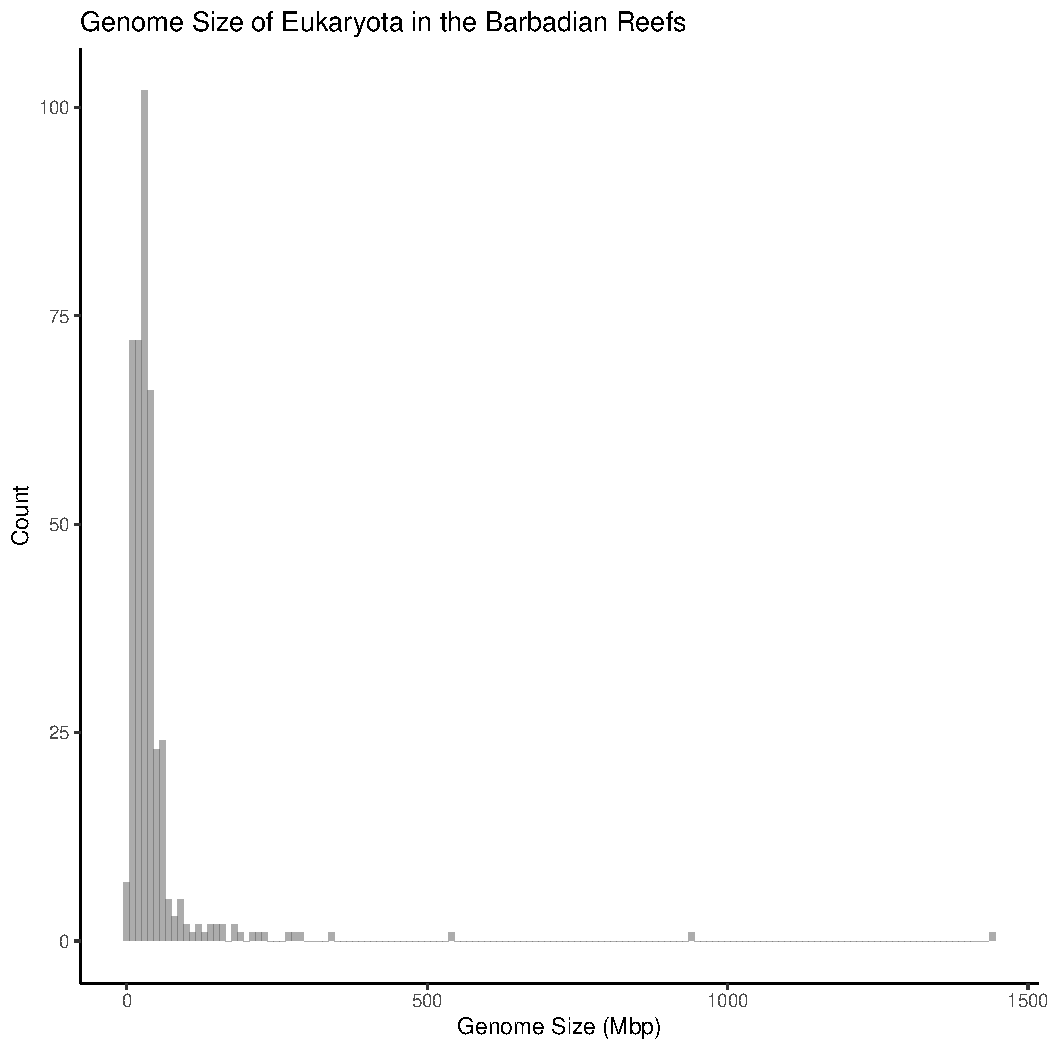
\includegraphics[width=\maxwidth]{figure/unnamed-chunk-7-1} 

\end{knitrout}


\begin{knitrout}
\definecolor{shadecolor}{rgb}{0.969, 0.969, 0.969}\color{fgcolor}\begin{kframe}
\begin{alltt}
\hlstd{euk} \hlkwb{<-} \hlkwd{induce_tree}\hlstd{(}\hlnum{2759}\hlstd{); euk}\hlopt{$}\hlstd{taxa} \hlkwb{<-} \hlstr{"Eukaryota"}
\hlstd{virus} \hlkwb{<-} \hlkwd{induce_tree}\hlstd{(}\hlnum{10239}\hlstd{); virus}\hlopt{$}\hlstd{taxa} \hlkwb{<-} \hlstr{"virus"}
\hlstd{bac} \hlkwb{<-} \hlkwd{induce_tree}\hlstd{(}\hlnum{2}\hlstd{) ; bac}\hlopt{$}\hlstd{taxa} \hlkwb{<-} \hlstr{"Bacteria"}
\hlstd{arch} \hlkwb{<-} \hlkwd{induce_tree}\hlstd{(}\hlnum{2157}\hlstd{); arch}\hlopt{$}\hlstd{taxa} \hlkwb{<-} \hlstr{"Archaea"}

\hlstd{everyone} \hlkwb{<-} \hlkwd{do.call}\hlstd{(}\hlstr{"rbind"}\hlstd{,} \hlkwd{list}\hlstd{(euk, virus, bac, arch))}

\hlstd{largest} \hlkwb{<-} \hlkwd{arrange}\hlstd{(everyone,}\hlkwd{desc}\hlstd{(genome_size))}

\hlstd{largest_species} \hlkwb{<-} \hlstd{largest[} \hlkwd{which}\hlstd{(largest}\hlopt{$}\hlstd{rank} \hlopt{==} \hlstr{"species"}\hlstd{), ]}

\hlkwd{library}\hlstd{(}\hlstr{"DescTools"}\hlstd{)}
\hlstd{largest_species}\hlopt{$}\hlstd{genome_size} \hlkwb{<-} \hlkwd{Winsorize}\hlstd{(largest_species}\hlopt{$}\hlstd{genome_size,} \hlkwc{maxval} \hlstd{=} \hlnum{50}\hlstd{,} \hlkwc{na.rm}\hlstd{=}\hlnum{TRUE}\hlstd{)}

\hlstd{p}\hlkwb{<-}\hlkwd{ggplot}\hlstd{(largest_species,} \hlkwd{aes}\hlstd{(}\hlkwc{x}\hlstd{=genome_size,} \hlkwc{fill}\hlstd{=taxa,} \hlkwc{color}\hlstd{=taxa))} \hlopt{+}
  \hlkwd{geom_histogram}\hlstd{(}\hlkwc{position}\hlstd{=}\hlstr{"identity"}\hlstd{,} \hlkwc{alpha}\hlstd{=}\hlnum{0.5}\hlstd{,} \hlkwc{binwidth} \hlstd{=} \hlnum{0.5}\hlstd{)} \hlopt{+}
  \hlkwd{labs}\hlstd{(}\hlkwc{title}\hlstd{=}\hlstr{"Genome Size of Cellular Organisms"} \hlstd{,}\hlkwc{x}\hlstd{=}\hlstr{"Genome Size (Mbp)"}\hlstd{,} \hlkwc{y} \hlstd{=} \hlstr{"Count"}\hlstd{)}\hlopt{+}
  \hlkwd{scale_color_brewer}\hlstd{(}\hlkwc{palette}\hlstd{=}\hlstr{"Dark2"}\hlstd{)}\hlopt{+}
  \hlkwd{scale_fill_brewer}\hlstd{(}\hlkwc{palette}\hlstd{=}\hlstr{"Dark2"}\hlstd{)}\hlopt{+}
  \hlkwd{theme_classic}\hlstd{()}
\hlstd{p}
\end{alltt}
\end{kframe}
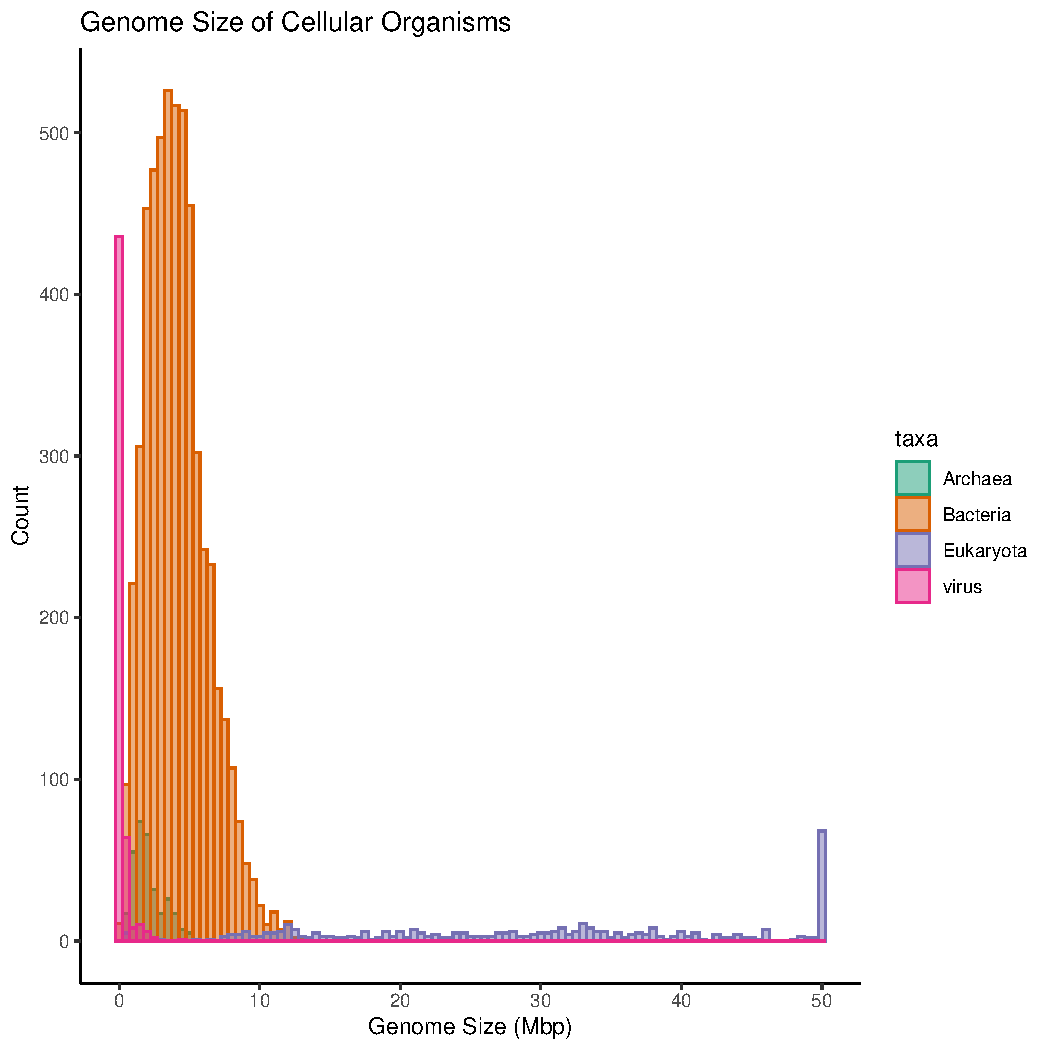
\includegraphics[width=\maxwidth]{figure/unnamed-chunk-8-1} 

\end{knitrout}

Now we repeat the above plot at the genus level rather than at the species level.
Although the two plots are very similar, we note that our calculation at each internal
nodes $t$ in the tree of life should be fixed.
Currently, we simply compute the average across all the children of $t$
but we should rather compute a weighted average.
As it is, the averaage genome size at or near the root is disportionality high because it
subject to a few large Eukaryota genomes

\begin{knitrout}
\definecolor{shadecolor}{rgb}{0.969, 0.969, 0.969}\color{fgcolor}\begin{kframe}
\begin{alltt}
\hlstd{largest_species} \hlkwb{<-} \hlstd{largest[} \hlkwd{which}\hlstd{(largest}\hlopt{$}\hlstd{rank} \hlopt{==} \hlstr{"genus"}\hlstd{), ]}
\hlstd{largest_species}\hlopt{$}\hlstd{genome_size} \hlkwb{<-} \hlkwd{Winsorize}\hlstd{(largest_species}\hlopt{$}\hlstd{genome_size,} \hlkwc{maxval} \hlstd{=} \hlnum{50}\hlstd{,} \hlkwc{na.rm}\hlstd{=}\hlnum{TRUE}\hlstd{)}

\hlstd{p}\hlkwb{<-}\hlkwd{ggplot}\hlstd{(largest_species,} \hlkwd{aes}\hlstd{(}\hlkwc{x}\hlstd{=genome_size,} \hlkwc{fill}\hlstd{=taxa,} \hlkwc{color}\hlstd{=taxa))} \hlopt{+}
  \hlkwd{geom_histogram}\hlstd{(}\hlkwc{position}\hlstd{=}\hlstr{"identity"}\hlstd{,} \hlkwc{alpha}\hlstd{=}\hlnum{0.5}\hlstd{,} \hlkwc{binwidth} \hlstd{=} \hlnum{0.5}\hlstd{)} \hlopt{+}
  \hlkwd{labs}\hlstd{(}\hlkwc{title}\hlstd{=}\hlstr{"Genome Size of Cellular Organisms"} \hlstd{,}\hlkwc{x}\hlstd{=}\hlstr{"Genome Size (Mbp)"}\hlstd{,} \hlkwc{y} \hlstd{=} \hlstr{"Count"}\hlstd{)}\hlopt{+}
  \hlkwd{scale_color_brewer}\hlstd{(}\hlkwc{palette}\hlstd{=}\hlstr{"Dark2"}\hlstd{)}\hlopt{+}
  \hlkwd{scale_fill_brewer}\hlstd{(}\hlkwc{palette}\hlstd{=}\hlstr{"Dark2"}\hlstd{)}\hlopt{+}
  \hlkwd{theme_classic}\hlstd{()}
\hlstd{p}
\end{alltt}
\end{kframe}
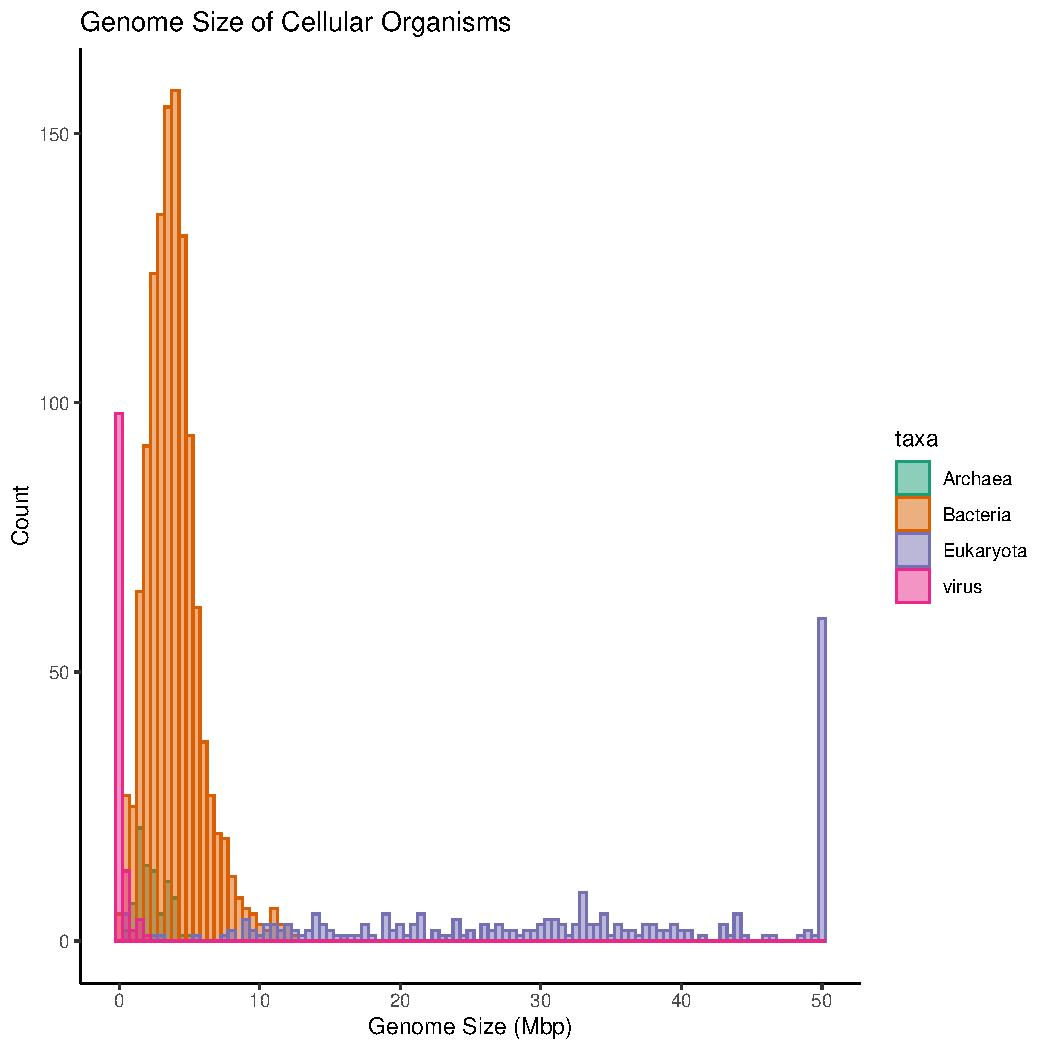
\includegraphics[width=\maxwidth]{figure/unnamed-chunk-9-1} 

\end{knitrout}


\section{Correlations between genome size and read count}

In this section, we look to see if there is a relationship between the number of reads that are mapped to an organism
and the size of the genome.
For this analysis, we will treat each superkingdom separately.


\begin{knitrout}
\definecolor{shadecolor}{rgb}{0.969, 0.969, 0.969}\color{fgcolor}\begin{kframe}
\begin{alltt}
\hlstd{euk} \hlkwb{<-} \hlkwd{induce_tree}\hlstd{(}\hlnum{2759}\hlstd{); euk}\hlopt{$}\hlstd{taxa} \hlkwb{<-} \hlstr{"Eukaryota"}
\hlstd{euk_species} \hlkwb{<-} \hlstd{euk[} \hlkwd{which}\hlstd{(euk}\hlopt{$}\hlstd{rank} \hlopt{==} \hlstr{"species"}\hlstd{), ]}
\hlstd{euk_species_a} \hlkwb{<-} \hlstd{euk_species; euk_species_a}\hlopt{$}\hlstd{site} \hlkwb{<-} \hlstr{"bellairs"}\hlstd{; euk_species_a}\hlopt{$}\hlstd{reads} \hlkwb{<-} \hlstd{euk_species}\hlopt{$}\hlstd{br_bel}
\hlstd{euk_species_b} \hlkwb{<-} \hlstd{euk_species; euk_species_b}\hlopt{$}\hlstd{site} \hlkwb{<-} \hlstr{"maycocks"}\hlstd{; euk_species_b}\hlopt{$}\hlstd{reads} \hlkwb{<-} \hlstd{euk_species}\hlopt{$}\hlstd{br_may}
\hlstd{euk_tmp} \hlkwb{<-} \hlkwd{rbind}\hlstd{(euk_species_a, euk_species_b)}
\hlkwd{ggplot}\hlstd{(euk_tmp,} \hlkwd{aes}\hlstd{(}\hlkwc{x}\hlstd{=}\hlkwd{log}\hlstd{(reads),} \hlkwc{y}\hlstd{=}\hlkwd{log}\hlstd{(genome_size),} \hlkwc{color} \hlstd{= site))} \hlopt{+}
  \hlkwd{geom_point}\hlstd{()} \hlopt{+} \hlkwd{geom_rug}\hlstd{()}\hlopt{+}  \hlkwd{geom_smooth}\hlstd{(}\hlkwc{method}\hlstd{=lm)} \hlopt{+}
  \hlkwd{stat_ellipse}\hlstd{()}
\end{alltt}
\end{kframe}
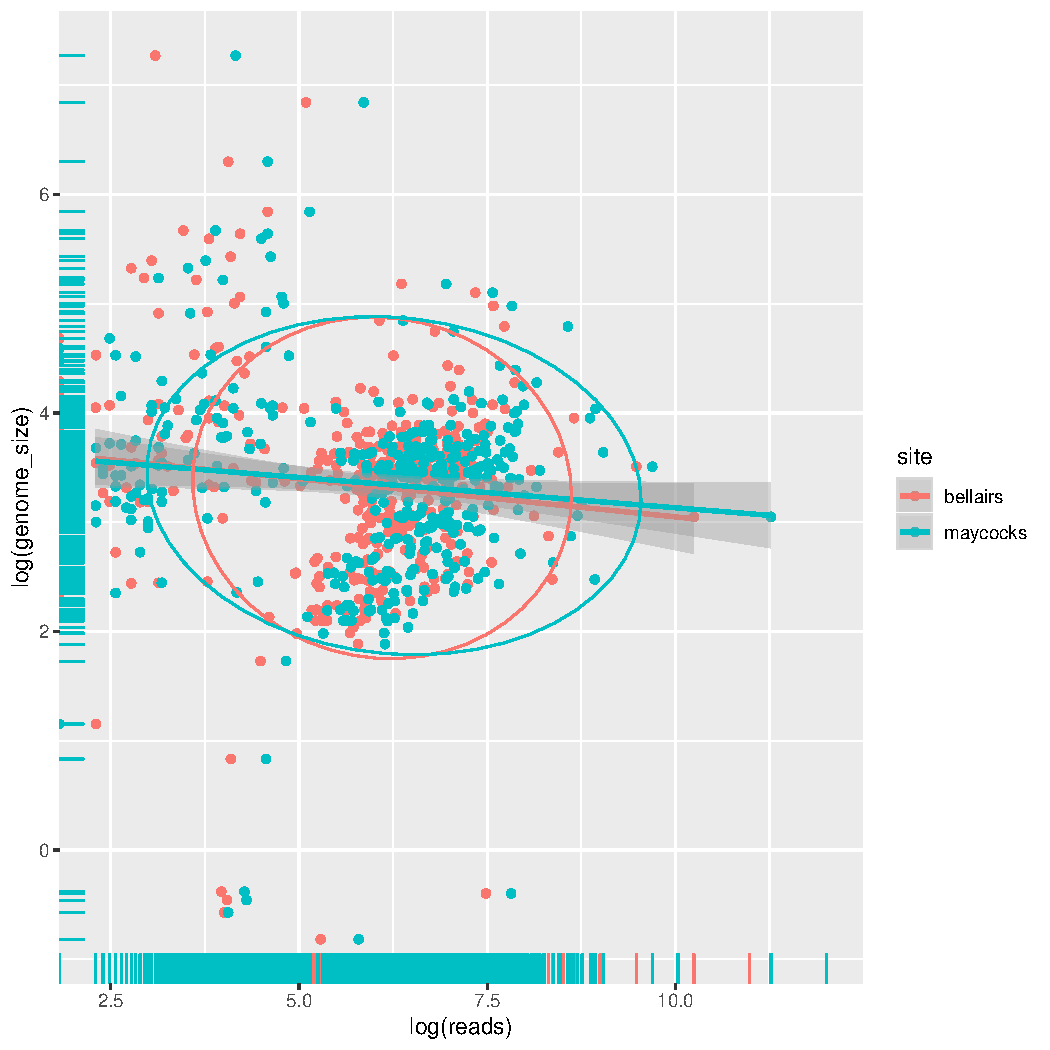
\includegraphics[width=\maxwidth]{figure/unnamed-chunk-10-1} 

\end{knitrout}

\begin{knitrout}
\definecolor{shadecolor}{rgb}{0.969, 0.969, 0.969}\color{fgcolor}\begin{kframe}
\begin{alltt}
\hlstd{virus} \hlkwb{<-} \hlkwd{induce_tree}\hlstd{(}\hlnum{10239}\hlstd{); virus}\hlopt{$}\hlstd{taxa} \hlkwb{<-} \hlstr{"virus"}
\hlstd{virus_species} \hlkwb{<-} \hlstd{virus[} \hlkwd{which}\hlstd{(virus}\hlopt{$}\hlstd{rank} \hlopt{==} \hlstr{"species"}\hlstd{), ]}
\hlstd{virus_species_a} \hlkwb{<-} \hlstd{virus_species; virus_species_a}\hlopt{$}\hlstd{site} \hlkwb{<-} \hlstr{"bellairs"}\hlstd{; virus_species_a}\hlopt{$}\hlstd{reads} \hlkwb{<-} \hlstd{virus_species}\hlopt{$}\hlstd{br_bel}
\hlstd{virus_species_b} \hlkwb{<-} \hlstd{virus_species; virus_species_b}\hlopt{$}\hlstd{site} \hlkwb{<-} \hlstr{"maycocks"}\hlstd{; virus_species_b}\hlopt{$}\hlstd{reads} \hlkwb{<-} \hlstd{virus_species}\hlopt{$}\hlstd{br_may}
\hlstd{virus_tmp} \hlkwb{<-} \hlkwd{rbind}\hlstd{(virus_species_a, virus_species_b)}
\hlkwd{ggplot}\hlstd{(virus_tmp,} \hlkwd{aes}\hlstd{(}\hlkwc{x}\hlstd{=}\hlkwd{log}\hlstd{(reads),} \hlkwc{y}\hlstd{=}\hlkwd{log}\hlstd{(genome_size),} \hlkwc{color} \hlstd{= site))} \hlopt{+}
  \hlkwd{geom_point}\hlstd{()} \hlopt{+} \hlkwd{geom_rug}\hlstd{()}\hlopt{+} \hlkwd{geom_smooth}\hlstd{(}\hlkwc{method}\hlstd{=lm)} \hlopt{+}
  \hlkwd{stat_ellipse}\hlstd{()}
\end{alltt}
\end{kframe}
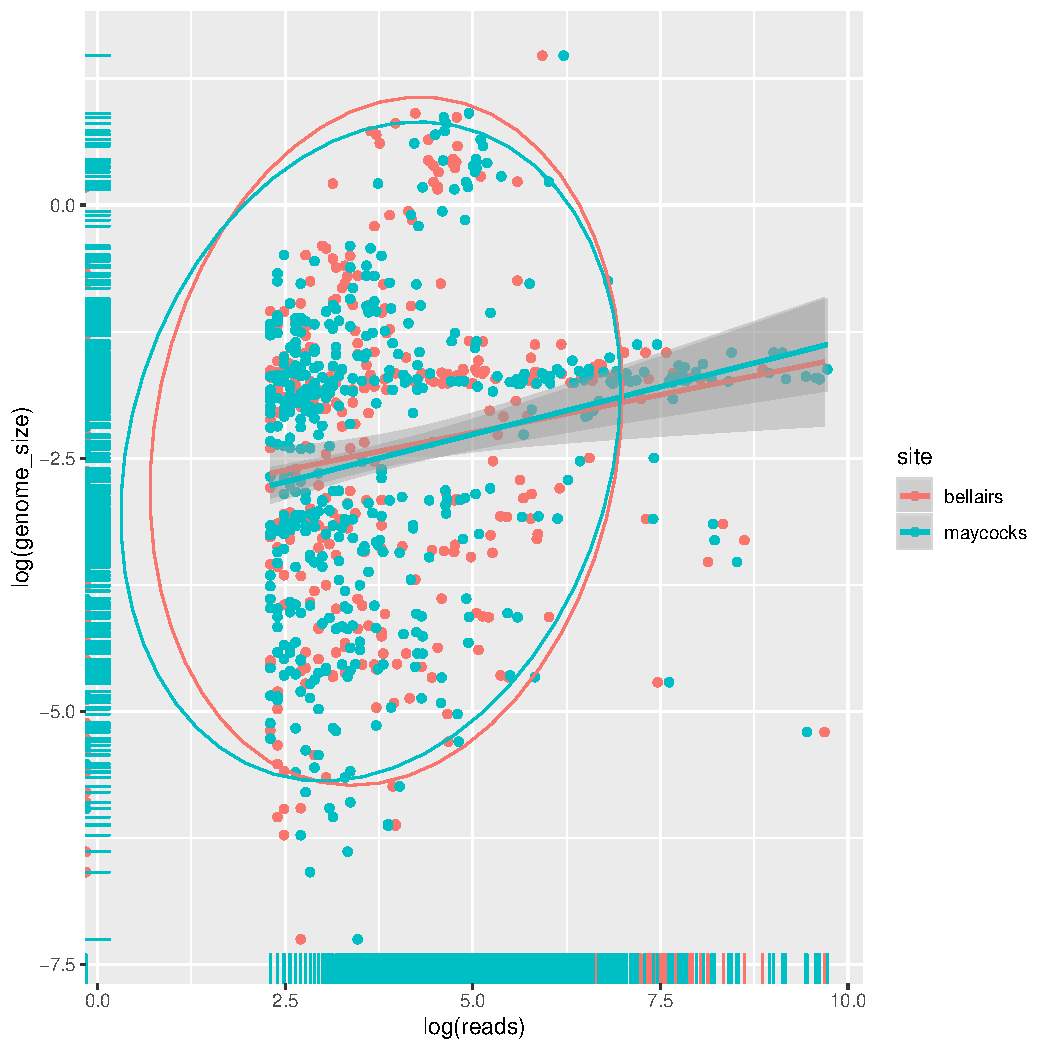
\includegraphics[width=\maxwidth]{figure/unnamed-chunk-11-1} 

\end{knitrout}

\begin{knitrout}
\definecolor{shadecolor}{rgb}{0.969, 0.969, 0.969}\color{fgcolor}\begin{kframe}
\begin{alltt}
\hlstd{bac} \hlkwb{<-} \hlkwd{induce_tree}\hlstd{(}\hlnum{2}\hlstd{) ; bac}\hlopt{$}\hlstd{taxa} \hlkwb{<-} \hlstr{"Bacteria"}
\hlstd{bac_species} \hlkwb{<-} \hlstd{bac[} \hlkwd{which}\hlstd{(bac}\hlopt{$}\hlstd{rank} \hlopt{==} \hlstr{"species"}\hlstd{), ]}
\hlstd{bac_species_a} \hlkwb{<-} \hlstd{bac_species; bac_species_a}\hlopt{$}\hlstd{site} \hlkwb{<-} \hlstr{"bellairs"}\hlstd{; bac_species_a}\hlopt{$}\hlstd{reads} \hlkwb{<-} \hlstd{bac_species}\hlopt{$}\hlstd{br_bel}
\hlstd{bac_species_b} \hlkwb{<-} \hlstd{bac_species; bac_species_b}\hlopt{$}\hlstd{site} \hlkwb{<-} \hlstr{"maycocks"}\hlstd{; bac_species_b}\hlopt{$}\hlstd{reads} \hlkwb{<-} \hlstd{bac_species}\hlopt{$}\hlstd{br_may}
\hlstd{bac_tmp} \hlkwb{<-} \hlkwd{rbind}\hlstd{(bac_species_a, bac_species_b)}
\hlkwd{ggplot}\hlstd{(bac_tmp,} \hlkwd{aes}\hlstd{(}\hlkwc{x}\hlstd{=}\hlkwd{log}\hlstd{(reads),} \hlkwc{y}\hlstd{=}\hlkwd{log}\hlstd{(genome_size),} \hlkwc{color} \hlstd{= site))} \hlopt{+}
  \hlkwd{geom_point}\hlstd{()} \hlopt{+} \hlkwd{geom_rug}\hlstd{()}\hlopt{+} \hlkwd{geom_smooth}\hlstd{(}\hlkwc{method}\hlstd{=lm)} \hlopt{+}
  \hlkwd{stat_ellipse}\hlstd{()}
\end{alltt}
\end{kframe}
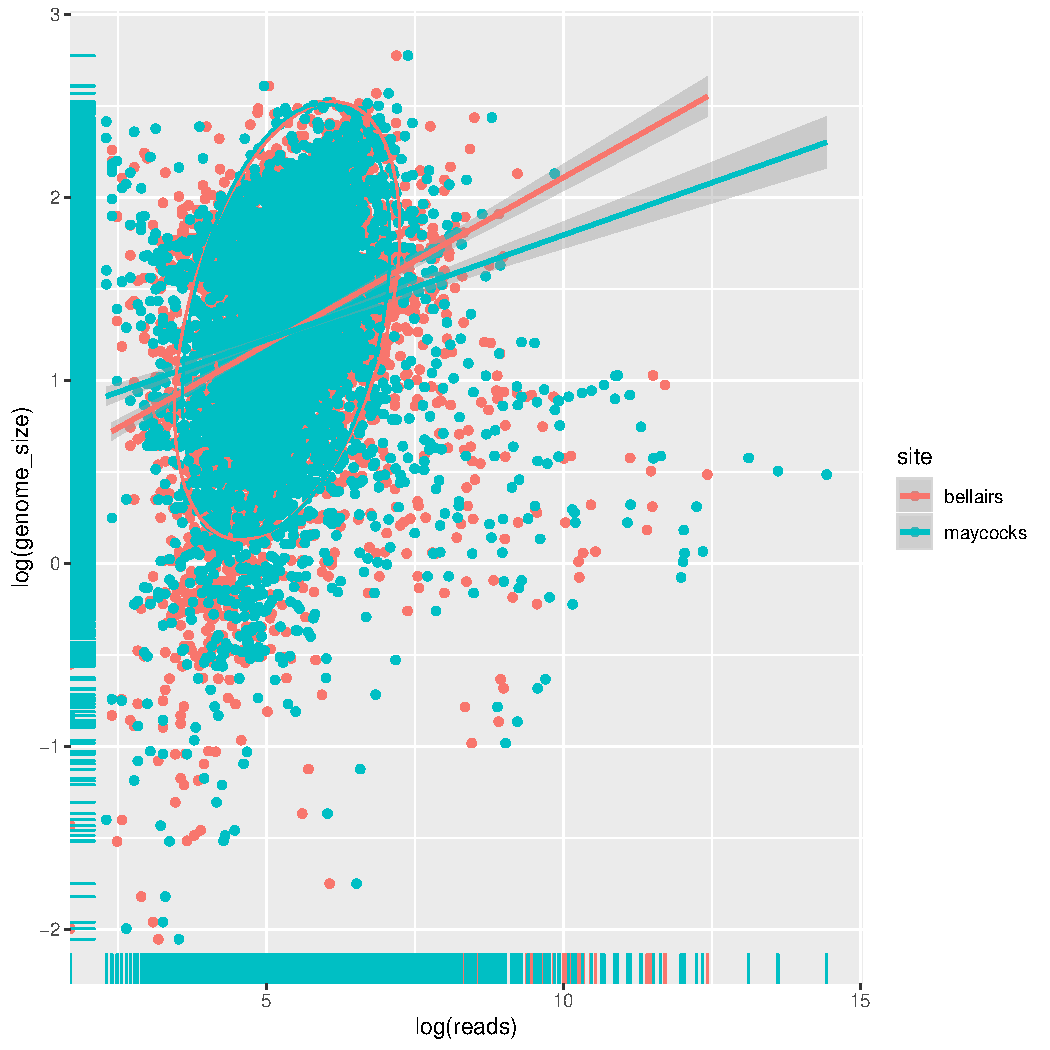
\includegraphics[width=\maxwidth]{figure/unnamed-chunk-12-1} 

\end{knitrout}

\begin{knitrout}
\definecolor{shadecolor}{rgb}{0.969, 0.969, 0.969}\color{fgcolor}\begin{kframe}
\begin{alltt}
\hlstd{arch} \hlkwb{<-} \hlkwd{induce_tree}\hlstd{(}\hlnum{2157}\hlstd{); arch}\hlopt{$}\hlstd{taxa} \hlkwb{<-} \hlstr{"Archaea"}
\hlstd{arch_species} \hlkwb{<-} \hlstd{arch[} \hlkwd{which}\hlstd{(arch}\hlopt{$}\hlstd{rank} \hlopt{==} \hlstr{"species"}\hlstd{), ]}
\hlstd{arch_species_a} \hlkwb{<-} \hlstd{arch_species; arch_species_a}\hlopt{$}\hlstd{site} \hlkwb{<-} \hlstr{"bellairs"}\hlstd{; arch_species_a}\hlopt{$}\hlstd{reads} \hlkwb{<-} \hlstd{arch_species}\hlopt{$}\hlstd{br_bel}
\hlstd{arch_species_b} \hlkwb{<-} \hlstd{arch_species; arch_species_b}\hlopt{$}\hlstd{site} \hlkwb{<-} \hlstr{"maycocks"}\hlstd{; arch_species_b}\hlopt{$}\hlstd{reads} \hlkwb{<-} \hlstd{arch_species}\hlopt{$}\hlstd{br_may}
\hlstd{arch_tmp} \hlkwb{<-} \hlkwd{rbind}\hlstd{(arch_species_a, arch_species_b)}
\hlkwd{ggplot}\hlstd{(arch_tmp,} \hlkwd{aes}\hlstd{(}\hlkwc{x}\hlstd{=}\hlkwd{log}\hlstd{(reads),} \hlkwc{y}\hlstd{=}\hlkwd{log}\hlstd{(genome_size),} \hlkwc{color} \hlstd{= site))} \hlopt{+}
  \hlkwd{geom_point}\hlstd{()} \hlopt{+} \hlkwd{geom_rug}\hlstd{()}\hlopt{+} \hlkwd{geom_smooth}\hlstd{(}\hlkwc{method}\hlstd{=lm)} \hlopt{+}
  \hlkwd{stat_ellipse}\hlstd{()}
\end{alltt}
\end{kframe}
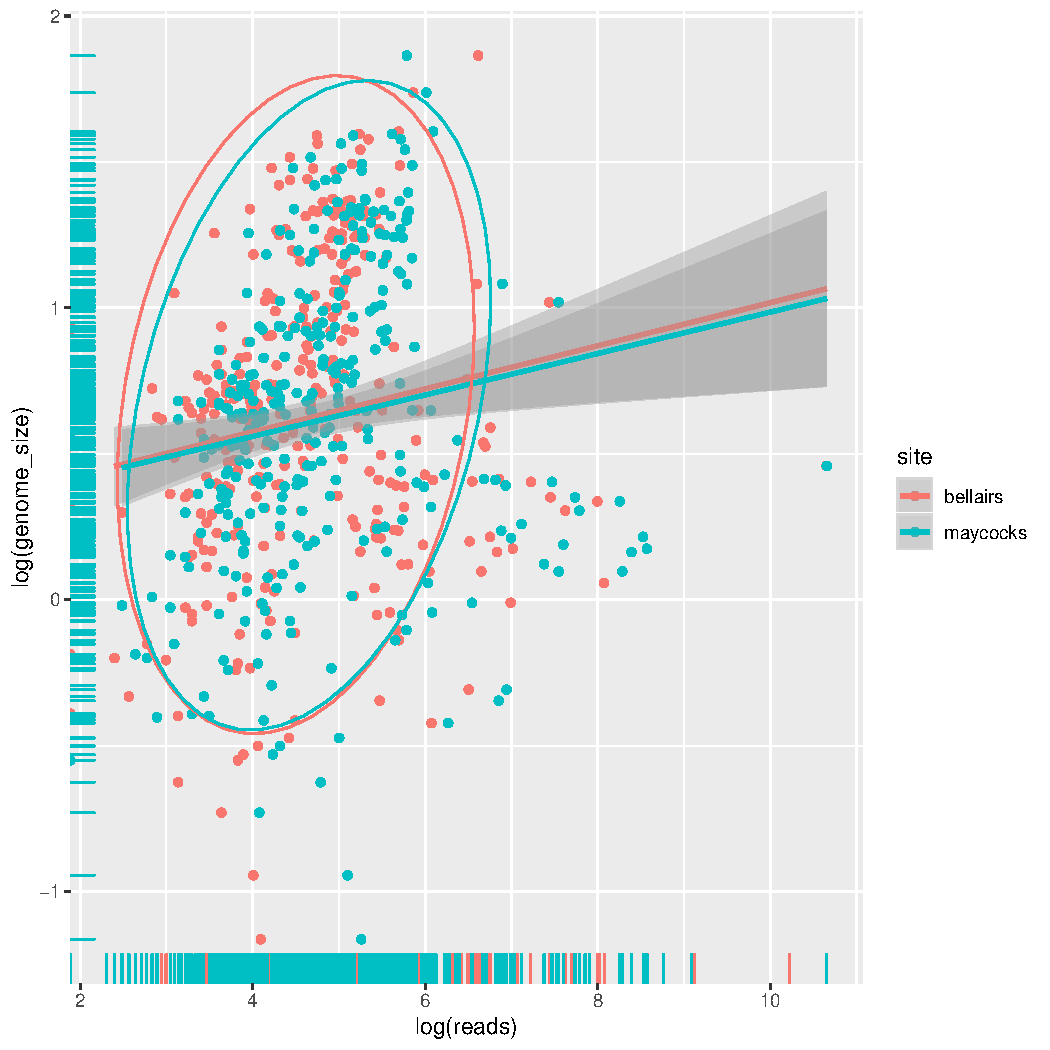
\includegraphics[width=\maxwidth]{figure/unnamed-chunk-13-1} 

\end{knitrout}



\section{Correcting for genome size}
To renormalize the counts what if we create a ratio based on the totals number of counts sequenced at specific location and divide it by the length of a genome size. A given organism's counts by that ratio. - Shawn





\subsection Attempting method mentioned above.
\begin{knitrout}
\definecolor{shadecolor}{rgb}{0.969, 0.969, 0.969}\color{fgcolor}\begin{kframe}
\begin{alltt}
bel_tot <- 4708322 \hlcom{#Tot # of BellairsCounts }
may_tot <- 10181105 \hlcom{#Tot # of MaycocksCounts}
\hlkwd{colnames}(gnempool)[6] <-\hlkwd{c}(\hlstr{"gn_size"})
gnempool$gn_size <- gnempool$gn_size * 1000000

\hlkwd{for} (i in 1:\hlkwd{nrow}(gnempool)) \{
    gnempool$renorm_bel_ratio[i] <- (bel_tot / gnempool$gn_size[i])
    gnempool$renorm_may_ratio[i] <- (may_tot / gnempool$gn_size[i])
    gnempool$renorm_bel_counts[i] <- (gnempool$renorm_bel_ratio[i] * gnempool$br_bel[i])
    gnempool$renorm_may_counts[i] <- (gnempool$renorm_may_ratio[i] * gnempool$br_may[i])
\}


\textbackslash{}end\{document\}
\end{alltt}


{\ttfamily\noindent\bfseries\color{errorcolor}{\#\# Error: <text>:14:1: unexpected input\\\#\# 13: \\\#\# 14: \textbackslash{}\\\#\#\ \ \ \  \textasciicircum{}}}\end{kframe}
\end{knitrout}
